\documentclass[12pt]{article}

\usepackage{ishn}

\makeindex[intoc]

\begin{document}

\hypersetup{pageanchor=false}
\begin{titlepage}
	\begin{center}
		\vspace*{1em}
		\Huge
		\textbf{III Combinatorics}

		\vspace{1em}
		\large
		Ishan Nath, Michaelmas 2024

		\vspace{1.5em}

		\Large

		Based on Lectures by Prof. Imre Leader

		\vspace{1em}

		\large
		\today
	\end{center}
	
\end{titlepage}
\hypersetup{pageanchor=true}

\tableofcontents

\newpage

%lecture 1

\setcounter{section}{-1}

\section{Introduction}%
\label{sec:intro}

We have the following list of things.
\begin{enumerate}[1:]
	\item Set systems.
	\item Isoperimetric inequalities.
	\item Intersection families.
\end{enumerate}

Books include `Combinatorics' by Bollob\'as, and `Combinatorics of Finite Sets', by Anderson.

\newpage

\section{Set Systems}%
\label{sec:ss}

Let $X$ be a set. A \emph{set system}\index{set system} on $X$, also called a family of subsets of $X$, is a family $\mathcal{A} \subseteq \mathcal{P}(X)$. For example,
\[
	X^{(r)} = \{A \subseteq X \mid |A| = r \}.
\]
Usually, $X = [n] = \{1, 2, \ldots, n\}$, so $|X^{(r)}| = \binom nr$. Thus,
\[
	[4]^{(2)} = \{12, 13, 14, 23, 24, 34\}.
\]

We make $\mathcal{P}(X)$ into a graph by joining $A$ and $B$ if $|A \triangle B| = 1$. This is the \emph{discrete cube}\index{discrete cube} $Q_n$.

Literally just a cube.

\[
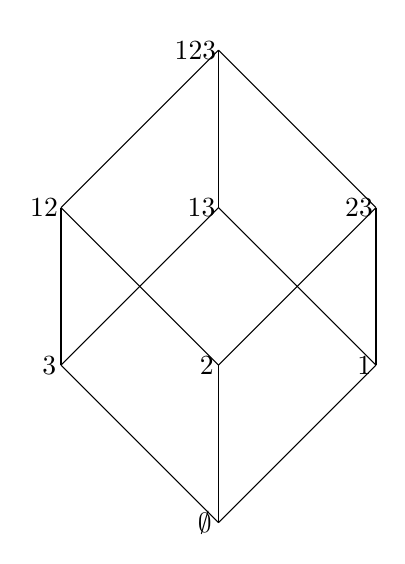
\begin{tikzpicture}[scale=2, every node/.style={circle, draw, fill=black, inner sep=0pt, minimum width=4pt}]

% Define the coordinates for the vertices of the cube
\coordinate (000) at (0,0);
\coordinate (001) at (1,1);
\coordinate (011) at (1,2);
\coordinate (010) at (0,1);
\coordinate (100) at (-1,1);
\coordinate (101) at (0,2);
\coordinate (111) at (0,3);
\coordinate (110) at (-1,2);

% Draw edges of the cube
\draw (000) -- (001);
\draw (001) -- (011);
\draw (011) -- (010);
\draw (010) -- (000);

\draw (100) -- (101);
\draw (101) -- (111);
\draw (111) -- (110);
\draw (110) -- (100);

\draw (000) -- (100);
\draw (001) -- (101);
\draw (011) -- (111);
\draw (010) -- (110);

% Place the vertices as small black circles

\node[draw=none, fill=none, anchor=east] at (000) {$\emptyset$};
\node[draw=none, fill=none, anchor=east] at (001) {1};
\node[draw=none, fill=none, anchor=east] at (011) {23};
\node[draw=none, fill=none, anchor=east] at (010) {2};
\node[draw=none, fill=none, anchor=east] at (100) {3};
\node[draw=none, fill=none, anchor=east] at (101) {13};
\node[draw=none, fill=none, anchor=east] at (111) {123};
\node[draw=none, fill=none, anchor=east] at (110) {12};

\end{tikzpicture}
\]
Alternatively, can view $Q_n$ as an $n$-dimensional unit cube $\{0, 1\}^n$, by identifying e.g. $\{1, 3\}$ with the binary string $101000\cdots$.
\[
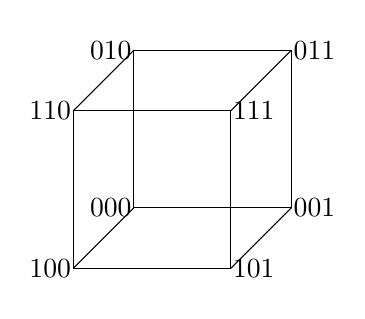
\begin{tikzpicture}[scale=2, every node/.style={circle, draw, fill=black, inner sep=0pt, minimum width=4pt}]

% Define the coordinates for the vertices of the cube
\coordinate (000) at (0,0,0);
\coordinate (001) at (1,0,0);
\coordinate (011) at (1,1,0);
\coordinate (010) at (0,1,0);
\coordinate (100) at (0,0,1);
\coordinate (101) at (1,0,1);
\coordinate (111) at (1,1,1);
\coordinate (110) at (0,1,1);

% Draw edges of the cube
\draw (000) -- (001);
\draw (001) -- (011);
\draw (011) -- (010);
\draw (010) -- (000);

\draw (100) -- (101);
\draw (101) -- (111);
\draw (111) -- (110);
\draw (110) -- (100);

\draw (000) -- (100);
\draw (001) -- (101);
\draw (011) -- (111);
\draw (010) -- (110);

% Place the vertices as small black circles

\node[draw=none, fill=none, anchor=east] at (000) {000};
\node[draw=none, fill=none, anchor=west] at (001) {001};
\node[draw=none, fill=none, anchor=west] at (011) {011};
\node[draw=none, fill=none, anchor=east] at (010) {010};
\node[draw=none, fill=none, anchor=east] at (100) {100};
\node[draw=none, fill=none, anchor=west] at (101) {101};
\node[draw=none, fill=none, anchor=west] at (111) {111};
\node[draw=none, fill=none, anchor=east] at (110) {110};


\end{tikzpicture}
\]

Say $\mathcal{A} \subseteq \mathcal{P}(X)$ is a \emph{chain}\index{chain} if, for all $A, B \in \mathcal{A}$, $A \subseteq B$ or $B \subseteq A$. For example,
\[
	\mathcal{A} = \{23, 12357, 1235, 123567\}
\]
is a chain.

Say $\mathcal{A}$ is an \emph{antichain}\index{antichain} if, for all $A, B \in \mathcal{A}$ and $A \neq B$, we have $A \not \subseteq B$. For example, $\mathcal{A} = \{23, 137\}$ is an antichain.

How large can a chain be? We can achieve $|\mathcal{A}| = n+1$ by taking
\[
	\mathcal{A} = \{ \emptyset, 1, 12, 123, \ldots, [n]\}
\]
Cannot beat this as each $0 \leq r \leq n$, $\mathcal{A}$ can contain at most one $r$-set (a member of $X^{(r)}$).

How large can an antichain be? We can achieve $|\mathcal{A}| = n$, e.g. $\mathcal{A} = \{1, 2, \ldots, n\}$. More generally, we can take $\mathcal{A} = X^{(r)}$, and the best is when $r = \lfloor n/2 \rfloor$.

% lecture 2

\begin{theorem}[Sperner's Lemma]
	Let $\mathcal{A} \subseteq \mathcal{P}(X)$ be an antichain. Then,
	\[
		|\mathcal{A}| \leq \binom{n}{\lfloor n/2 \rfloor}.
	\]
\end{theorem}

The idea is follows: we know that a chain meets a layer in at most one point, since a layer is an antichain. If we decompose the cube into chains, we have at most one element of an antichain in each chain.

\begin{proofbox}
	We will decompose $\mathcal{P}(X)$ into $\binom n {\lfloor n/2 \rfloor}$ chains, then we are done. To achieve this, it is sufficient to find:
	\begin{enumerate}[(i)]
		\item For each $r < n/2$, a matching from $X^{(r)}$ to $X^{(r + 1)}$.
		\item For each $r \geq n/2$, a matching from $X^{(r)}$ to $X^{(r - 1)}$.
	\end{enumerate}
	Then we put these together to form our chains; each passing through $X^{(\lfloor n/2 \rfloor)}$.

	By taking complements, it is enough to prove (i).

	Let $G$ be the bipartite subgraph of $Q_n$ spanned by $X^{(r)} \cup X^{(r + 1)}$: we seek a matching from $X^{(r)}$ to $X^{(r + 1)}$.

	For any $S \subseteq X^{(r)}$, the number of edges from $S$ to $\Gamma(S)$ is $|S|(n - r)$, since each edge in $S$ has $n - r$ edges.

	Moreover there are at most $|\Gamma(S)|(r + 1)$ edges, counting from $\Gamma(S)$. Therefore,
	\[
	|\Gamma(S)| \geq \frac{|S|(n-r)}{r + 1} \geq |S|.
	\]
	So we are done, by Hall's matching theorem.
\end{proofbox}

\begin{center}
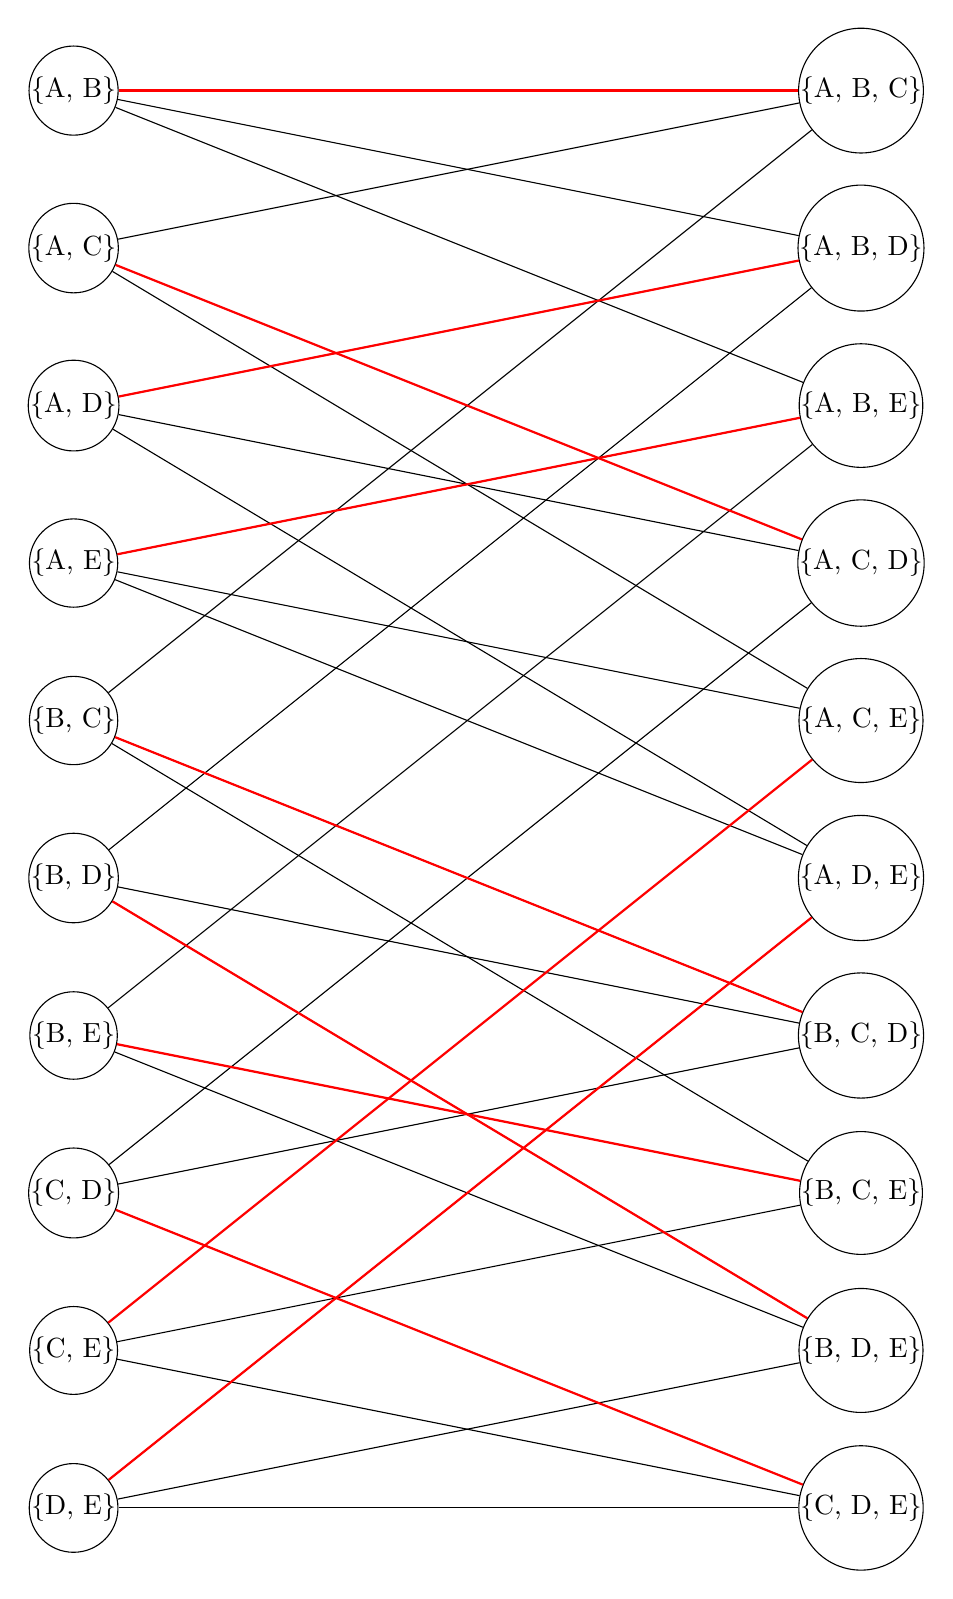
\begin{tikzpicture}[scale=1,>=latex, every node/.style={circle, draw, minimum size=1mm, inner sep=0pt}]

    % Define the 2-element subsets X^{(2)} (left side)
    \node (AB) at (-5, 9) {\{A, B\}};
    \node (AC) at (-5, 7) {\{A, C\}};
    \node (AD) at (-5, 5) {\{A, D\}};
    \node (AE) at (-5, 3) {\{A, E\}};
    \node (BC) at (-5, 1) {\{B, C\}};
    \node (BD) at (-5, -1) {\{B, D\}};
    \node (BE) at (-5, -3) {\{B, E\}};
    \node (CD) at (-5, -5) {\{C, D\}};
    \node (CE) at (-5, -7) {\{C, E\}};
    \node (DE) at (-5, -9) {\{D, E\}};

    % Define the 3-element subsets X^{(3)} (right side)
    \node (ABC) at (5, 9) {\{A, B, C\}};
    \node (ABD) at (5, 7) {\{A, B, D\}};
    \node (ABE) at (5, 5) {\{A, B, E\}};
    \node (ACD) at (5, 3) {\{A, C, D\}};
    \node (ACE) at (5, 1) {\{A, C, E\}};
    \node (ADE) at (5, -1) {\{A, D, E\}};
    \node (BCD) at (5, -3) {\{B, C, D\}};
    \node (BCE) at (5, -5) {\{B, C, E\}};
    \node (BDE) at (5, -7) {\{B, D, E\}};
    \node (CDE) at (5, -9) {\{C, D, E\}};

    % Draw edges representing the bipartite connections (subset relationships)
    \draw (AB) -- (ABC);
    \draw (AB) -- (ABD);
    \draw (AB) -- (ABE);

    \draw (AC) -- (ABC);
    \draw (AC) -- (ACD);
    \draw (AC) -- (ACE);

    \draw (AD) -- (ABD);
    \draw (AD) -- (ACD);
    \draw (AD) -- (ADE);

    \draw (AE) -- (ABE);
    \draw (AE) -- (ACE);
    \draw (AE) -- (ADE);

    \draw (BC) -- (ABC);
    \draw (BC) -- (BCD);
    \draw (BC) -- (BCE);

    \draw (BD) -- (ABD);
    \draw (BD) -- (BCD);
    \draw (BD) -- (BDE);
    \draw (BE) -- (ABE);
    \draw (BE) -- (BCE);
    \draw (BE) -- (BDE);
    \draw (CD) -- (ACD);
    \draw (CD) -- (BCD);
    \draw (CD) -- (CDE);
    \draw (CE) -- (ACE);
    \draw (CE) -- (BCE);
    \draw (CE) -- (CDE);
    \draw (DE) -- (ADE);
    \draw (DE) -- (BDE);
    \draw (DE) -- (CDE);

    % Draw the matching edges
    \draw[red,thick] (AB) -- (ABC);
    \draw[red,thick] (AC) -- (ACD);
    \draw[red,thick] (AD) -- (ABD);
    \draw[red,thick] (AE) -- (ABE);
    \draw[red,thick] (BC) -- (BCD);
    \draw[red,thick] (BD) -- (BDE);
    \draw[red,thick] (BE) -- (BCE);
    \draw[red,thick] (CD) -- (CDE);
    \draw[red,thick] (CE) -- (ACE);
    \draw[red,thick] (DE) -- (ADE);

\end{tikzpicture}
\end{center}

When do we have equality in Sperner's? The above proof tells us nothing.

Our aim is to prove the following: if $\mathcal{A}$ is an antichain, then
\[
\sum_{r = 0}^n \frac{|\mathcal{A} \cap X^{(r)}|}{\binom nr} \leq 1.
\]
In other words, the percentages of each layer occupied add up to at most 1. This trivially implies Sperner's.

\subsection{Shadows}%
\label{sub:shadow}

For $\mathcal{A} \subseteq X^{(r)}$, the \emph{shadow}\index{shadow} of $\mathcal{A}$ is $\partial \mathcal{A} = \partial^- \mathcal{A} \subseteq X^{(r - 1)}$ defined by
\[
	\partial \mathcal{A} = \{ B \in X^{(r-1)} \mid B \subseteq A \text{ for some } A \in \mathcal{A}\}.
\]
For example, if $\mathcal{A} = \{123, 124, 134, 137\}$, then
\[
	\partial \mathcal{A} = \{12, 13, 23, 14, 24, 34, 17, 37\}.
\]

\begin{proposition}[Local LYM]
	Let $\mathcal{A} \subseteq X^{(r)}$. Then,
	\[
		\frac{|\partial \mathcal{A}|}{\binom{n}{r-1}} \geq \frac{|\mathcal{A}|}{\binom{n}{r}}.
	\]
\end{proposition}

So, the fraction of the local occupancy by $\partial \mathcal{A}$, is at least the occupancy by $\mathcal{A}$.

\begin{remark}
	LYM = Lubell, Meshalkin, Yamamoto.
\end{remark}

\begin{proofbox}
	We look at the number of $\mathcal{A}$ to $\partial \mathcal{A}$ edges in the bipartite graph $Q_n$; counting from above, there are exactly $|\mathcal{A}| r$.

	However counting from below, it is at most $|\partial \mathcal{A}|(n - r + 1)$. So,
	\[
		\frac{|\partial \mathcal{A}|}{|\mathcal{A}|} \geq \frac{r}{n - r + 1} = \frac{\binom n{r-1}}{\binom nr}.
	\]
	So we are done.
\end{proofbox}

\begin{remark}
	When do we have equality? We lose equality if an element in $\partial \mathcal{A}$ is connected to an element not in $\mathcal{A}$, so for this not to occur, we need that for all $A \in \mathcal{A}$, and $i \in A$, $j \not \in \mathcal{A}$, that $A - \{i\} \cup \{j\} \in \mathcal{A}$.

	But this is very strong, and in fact either $\mathcal{A} = \emptyset$ or $X^{(r)}$.
\end{remark}

\begin{theorem}[LYM Inequality]
	Let $A \subseteq \mathcal{P}(X)$ be an antichain. Then,
	\[
	\sum_{r = 0}^n \frac{|\mathcal{A} \cap X^{(r)}|}{\binom nr} \leq 1.
	\]
\end{theorem}

As a bit of notation, we write $\mathcal{A}_r$ for $\mathcal{A} \cap X^{(r)}$.

We will look at two proofs. The first idea is to bubble down with local LYM.

\begin{proofbox}
	Obviously
	\[
	\frac{|\mathcal{A}_n|}{\binom nn} \leq 1.
	\]
	Now, $\partial A_n$ and $\mathcal{A}_{n-1}$ are disjoint, as $\mathcal{A}$ is an antichain. So,
	\[
		\frac{|\partial \mathcal{A}_n|}{\binom n{n-1}} + \frac{|\mathcal{A}_{n-1}|}{\binom n{n-1}} = \frac{|\partial \mathcal{A}_n \cup \mathcal{A}_{n-1}|}{\binom n{n-1}} \leq 1,
	\]
	whence we get
	\[
		\frac{|\mathcal{A}_n|}{\binom nn} + \frac{|\mathcal{A}_{n-1}|}{\binom n{n-1}} \leq 1,
	\]
	by local LYM. We now continue again. Notice $\partial (\partial \mathcal{A}_n \cup \mathcal{A}_{n-1})$ is disjoint from $\mathcal{A}_{n-2}$, we find
	\[
		\frac{|\partial(\partial \mathcal{A}_n \cup \mathcal{A}_{n-1})|}{\binom n{n-2}} + \frac{|\mathcal{A}_{n-2}|}{\binom n{n-2}} \leq 1,
	\]
	whence
	\[
		\frac{|\partial \mathcal{A}_n \cup \mathcal{A}_{n-1}|}{\binom n{n-1}} + \frac{|\mathcal{A}_{n-2}|}{\binom n{n-2}} \leq 1.
	\]
	We can now continue inductively.
\end{proofbox}

When do we have equality? We must have had equality in each use of local LYM. Hence equality in LYM needs that the maximum $r$ with $\mathcal{A}_r \neq \emptyset$, then $\mathcal{A}_r = X^{(r)}$.

Hence equality in Sperner needs either $\mathcal{A} = X^{(n/2)}$, if $n$ is even, or $\mathcal{A} = X^{(\lfloor n/2 \rfloor)}$ or $X^{(\lceil n/2 \rceil)}$, for $n$ odd.

% lecture 3

Now time for another proof.

\begin{proofbox}
	Choose uniformly at random a maximal chain $\mathcal{C}$. For any $r$-set $A$, note that
	\[
	\mathbb{P}(A \in \mathcal{C}) = \frac{1}{\binom nr}.
	\]
	So for our antichain $\mathcal{A}$,
	\[
		\mathbb{P}(\mathcal{C} \text{ meets } \mathcal{A}_r) = \frac{|\mathcal{A}_r|}{\binom nr},
	\]
	as these events are disjoint. Hence, since $\mathcal{C}$ can meet $\mathcal{A}$ at one point at most,
	\[
		\mathbb{P}(\mathcal{C} \text{ meets } \mathcal{A}) = \sum_{r = 0}^n \frac{|\mathcal{A}_r|}{\binom nr},
	\]
	from which we get
	\[
	\sum_{r = 0}^n \frac{|\mathcal{A}_r|}{\binom nr} \leq 1.
	\]
\end{proofbox}

Equivalently, the number of maximal chains is $n!$, and the number through any fixed $r$-set is $r!(n-r)!$, so
\[
\sum_r |\mathcal{A}_r| r! (n-r)! \leq n!.
\]

We now return to shadows. For $\mathcal{A} \subseteq X^{(r)}$, we have
\[
|\partial \mathcal{A}| \geq |\mathcal{A}| \frac{r}{n - r + 1}.
\]
We know that equality is rare: it only happens for $\mathcal{A} = \emptyset$, or $X^{(r)}$. What happens in between?

In other words, given $|\mathcal{A}|$, how should we choose $\mathcal{A} \subseteq X^{(r)}$ to minimise $|\partial \mathcal{A}|$?

It is believable that if $|\mathcal{A}| = \binom kr$, then we should take $\mathcal{A} = [k]^{(r)}$. In between adjacent binomials, it is believable that we should take $[k]^{(r)}$, plus some $r$-sets in $[k+1]^{(r)}$.

\begin{exbox}
	For $\mathcal{A} \subseteq X^{(3)}$ with 
	\[
	|\mathcal{A}| = \binom 83 + \binom 42,
	\]
	we could take
	\[
		\mathcal{A} = [8]^3 \cup \{9 \cup B \mid B \in [4]^{(2)}\}.
	\]
\end{exbox}

In some ways our set $\mathcal{A}$ should be of minimal `order', under some ordering on $X^{(r)}$.

\subsection{Total Orders}%
\label{sub:to_xr}

Let $A, B$ be distinct $r$-sets, and say $A = a_1 \ldots a_r$, $B = b_1 \ldots b_r$, where $a_1 < \cdots < a_r$, $b_1 < \cdots < a_r$.

We say that $A < B$ in the \emph{lexographic}\index{lexographic ordering} or \emph{lex} ordering if for some $j$ we have $a_i = b_i$ for all $i < j$, and $a_j < b_j$. So lex cares about small elements.

\begin{exbox}
	Lex on $[4]^{(2)}$ orders the elements as $12, 13, 14, 23, 24, 34$.

	Lex on $[6]^{(3)}$ orders the elements as
	\begin{align*}
		123, &124, 125, 126, 134, 135, 136, 145, 146, 156, \\
		     &234, 235, 236, 245, 246, 256, 345, 346, 356, 456.
	\end{align*}
\end{exbox}

We say that $A < B$ in the \emph{colexographic}\index{colexographic ordering} or \emph{colex} ordering if for some $j$, we have $a_i = b_i$ for all $i > j$, and $a_j < b_j$. So colex cares about big elements.


\begin{exbox}
	Colex on $[4]^{(2)}$ orders the elements as $12, 13, 23, 14, 24, 34$.

	Colex on $[6]^{(3)}$ orders the elements as
	\begin{align*}
		123, &124, 134, 234, 125, 135, 235, 145, 245, 345, \\
		     &126, 136, 236, 146, 246, 346, 156, 256, 356, 456.
	\end{align*}
\end{exbox}

Note that in colex, $[n-1]^{(r)}$ is an initial segment of $[n]^{(r)}$. This is not true in lex.

This allows us to view colex as an enumeration of $\mathbb{N}^{(r)}$.

\begin{remark}
	$A < B$ in colex $\iff A^c < B^c$ in lex, with ground set ordering ordering reversed.
\end{remark}

Colex in particular may be the ordering we want to solve the above problem, minimizing $|\partial \mathcal{A}|$. Our aim will then be to show that initial segments of colex are the best for $\partial$, i.e. if $\mathcal{A} \subseteq X^{(r)}$ and $\mathcal{C} \subseteq X^{(r)}$ is the initial segment of colex with $|\mathcal{C}| = |\mathcal{A}|$, then
\[
|\partial \mathcal{C}| \leq |\partial \mathcal{A}|.
\]
In particular,
\[
	|\mathcal{A}| = \binom kr \implies |\partial \mathcal{A}| = \binom k{r-1}.
\]
\subsection{Compression}%
\label{sub:comp}

The idea is to try to transform $\mathcal{A} \subseteq X^{(r)}$ into some $\mathcal{A}\ \subseteq X^{(r)}$ such that:
\begin{enumerate}[(i)]
	\item $|\mathcal{A}'| = |\mathcal{A}|$.
	\item $|\partial \mathcal{A}'| \leq |\partial \mathcal{A}|$.
	\item $\mathcal{A}'$ looks more like $\mathcal{C}$ than $\mathcal{A}$ did.
\end{enumerate}

Ideally, we would like a family of such `compressions'
\[
\mathcal{A} \to \mathcal{A}' \to \cdots \to \mathcal{B},
\]
such that either $\mathcal{B} = \mathcal{C}$, or $\mathcal{B}$ is so similar to $\mathcal{C}$ that we can directly check that
\[
|\partial \mathcal{B}| \geq |\partial \mathcal{C}|.
\]

% lecture 4

The fact that colex prefers 1 to 2 inspires the following: fix $1 \leq i < j \leq n$. The \emph{$ij$-compression}\index{compression} $C_{ij}$ is defined as follows:

For $A \in X^{(r)}$, set
\[
C_{ij}(A) =
\begin{cases}
	A \cup i - j &\text{if $j \in A$, $i \not \in A$ },\\
	A &\text{else.}
\end{cases}
\]
For $\mathcal{A} \subseteq X^{(r)}$, set
\[
	C_{ij}(\mathcal{A}) = \{ C_{ij}(A) \mid A \in \mathcal{A}\} \cup \{A \in \mathcal{A} \mid C_{ij}(A) \in \mathcal{A}\}.
\]
%For example, ....
So $C_{ij}(\mathcal{A}) \subseteq X^{(r)}$, and $|C_{ij}(\mathcal{A})| = |\mathcal{A}|$. Say $\mathcal{A}$ is $ij$-compressed if $C_{ij}(\mathcal{A}) = \mathcal{A}$.

\begin{lemma}
	Let $\mathcal{A} \subseteq X^{(r)}$, and $1 \leq i < j \leq n$. Then
	\[
	|\partial C_{ij}(\mathcal{A})| \leq |\partial\mathcal{A}|.
	\]
\end{lemma}

\begin{proofbox}
	Write $\mathcal{A}'$ for $C_{ij}(\mathcal{A})$, and let $B \in \partial \mathcal{A}' - \partial \mathcal{A}$. We will show that $i \in B, j \not \in B$, and $B \cup j - i \in \partial \mathcal{A} - \partial \mathcal{A}'$, which will show that we are done.

	We have that $B \cup x \in \mathcal{A}'$, for some $x$, with $B \cup x \not \in \mathcal{A}$. So, $i \in B \cup x$, $j \not \in B \cup x$, and $(B \cup x) \cup j - i \in \mathcal{A}$.

	We cannot have $x = i$, otherwise $(B \cup x) \cup j - i = B \cup j$, giving $B \in \partial \mathcal{A}$. So $i \in B$, and $j \not \in B$.

	Also, notice $B \cup j - i \in \partial \mathcal{A}$, since $(B \cup x) \cup j - i \in \mathcal{A}$.

	Suppose $B \cup j - i \in \partial \mathcal{A}'$, so $(B \cup j - i) \cup y \in \mathcal{A}'$ for some $y$. We cannot have $y = i$, else $B \cup j \in \mathcal{A}'$, so $B \cup j \in \mathcal{A}$, contradicting $B \not \in \partial \mathcal{A}$. So $j \in (B \cup j - i) \cup y$, and $i \not \in (B \cup j - i) \cup y$.

	Whence both $(B \cup j - i) \cup y$ and $B \cup y$ belong to $\mathcal{A}$, by definition of $\mathcal{A}'$, contradicting $B \not \in \partial \mathcal{A}$.
\end{proofbox}

\begin{remark}
	We have actually shown that $\partial C_{ij}(\mathcal{A}) \subseteq C_{ij} \partial \mathcal{A}$.
\end{remark}

Say $\mathcal{A} \subseteq X^{(r)}$ is \emph{left-compressed}\index{left-compressed} if $C_{ij}(\mathcal{A}) = \mathcal{A}$ for all $i \leq j$.

\begin{corollary}
	Let $\mathcal{A} \subseteq X^{(r)}$. Then there exists a left-compressed $\mathcal{B} \subseteq X^{(r)}$ with $|\mathcal{B}| = |\mathcal{A}|$, and $|\partial \mathcal{B}| \leq |\partial \mathcal{A}|$.
\end{corollary}

\begin{proofbox}
	Define a sequence $\mathcal{A}_0, \mathcal{A}_1, \ldots$ as follows. Let $\mathcal{A}_0 = \mathcal{A}$.

	Having defined $\mathcal{A}_0, \ldots, \mathcal{A}_k$, if $\mathcal{A}_k$ is left-compressed then we can stop the sequence with $\mathcal{A}_k$.

	If not, choose $i < j$ such that $\mathcal{A}_j$ is not $ij$-compresssed, and set $\mathcal{A}_{k+1} = C_{ij}(\mathcal{A}_k)$.

	This must terminate, as for example
	\[
	\sum_{A \in \mathcal{A}_k} \sum_{i \in A} i
	\]
	is strictly decreasing in $k$.

	Then the final term $\mathcal{B} = \mathcal{A}_k$ satisfies that $|\mathcal{B}| = |\mathcal{A}|$, and $|\partial \mathcal{B}| \leq |\partial \mathcal{A}|$, by the previous lemma.
\end{proofbox}

\begin{remark}
	\begin{enumerate}
		\item[]
		\item Similarly we may choose all $\mathcal{B} \subseteq X^{(r)}$ with $|\mathcal{B}| = |\mathcal{A}|$, and $|\partial \mathcal{B}| \leq |\partial \mathcal{A}|$, and then choose one with smallest sum of elements.
		\item We can choose the order of the $C_{ij}$ so that no $C_{ij}$ is applied twice.
		\item Any initial segment of colex is left-compressed. The converse is false, for example lex: $\{123, 124, 125, 126\}$.
	\end{enumerate}	
\end{remark}

This is not exactly what we want; we want to show that this is colex.

The fact that colex prefers 23 to 14 inspires the following. Let $U, V \subseteq X$ with $|U| = |V|$, $U \cap V = \emptyset$, and $\max V > \max U$.

Define the \emph{$UV$-compression}\index{compression} as follows: for $A \subseteq X$,
\[
C_{UV}(A) =
\begin{cases}
	A \cup U - V & \text{if $V \subseteq A$, $U \cap A = \emptyset$}, \\
	A &\text{otherwise}.
\end{cases}
\]
For $\mathcal{A}\subseteq X^{(r)}$, set
\[
	C_{UV}(\mathcal{A}) = \{C_{UV}(A) \mid A \in \mathcal{A}\} \cup \{A \in \mathcal{A} \mid C_{UV}(A) \in \mathcal{A}\}.
\]
For example if $\mathcal{A} = \{123, 124, 147, 237, 238, 149\}$, then
\[
C_{23, 14}(\mathcal{A}) = \{123, 124, 147, 237, 238, 239\}.
\]
So $C_{UV}(\mathcal{A}) \subseteq X^{(r)}$, and $|C_{UV}(\mathcal{A})| = |\mathcal{A}|$. Say $\mathcal{A}$ is \emph{$UV$-compressed} if $C_{UV}(\mathcal{A}) = \mathcal{A}$.

Sadly, we can have $|\partial C_{UV}(\mathcal{A})| > |\partial \mathcal{A}|$. For example if $\mathcal{A} = \{147, 137\}$, then $|\partial \mathcal{A}| = 5$, but $C_{23,14}(\mathcal{A}) = \{237, 147\}$ has $|\partial C_{23, 14}(\mathcal{A})| = 6$.

We can prove the following at least:

\begin{lemma}
	Let $\mathcal{A} \subseteq X^{(r)}$ be $UV$-compressed for all $U, V$ with $|U| = |V|$, $U \cap V = \emptyset$ and $\max V > \max U$. Then $\mathcal{A}$ is an initial segment of colex.
\end{lemma}

\begin{proofbox}
	Suppose not. Then there exists $A, B \in X^{(r)}$ with $B < A$ in colex, but $A \in \mathcal{A}$, $B \not \in \mathcal{A}$. 

	Set $V = A \setminus B$, $U = B \setminus A$. Then clearly $|V| = |U|$, and $U, V$ are disjoint, with $\max V > \max U$ since $B < A$. So, $C_{UV}(A) = B$, contradicting $\mathcal{A}$ $UV$-compressed.
\end{proofbox}

% lecture 5

But we can show the following:

\begin{lemma}
	Let $U, V \subseteq X$ with $|U| = |V|$, $U \cap V = \emptyset$, and $\max U < \max V$. For $\mathcal{A} \subseteq X^{(r)}$, suppose that for all $u$, there exists $v$ such that $\mathcal{A}$ is $(U - u, V - v)$-compressed. Then,
	\[
	|\partial C_{UV}(\mathcal{A})| \leq |\partial \mathcal{A}|.
	\]
\end{lemma}

\begin{proofbox}
	Let $\mathcal{A}' = C_{UV}(\mathcal{A})$. For $B \in \partial \mathcal{A}' - \partial \mathcal{A}$, we will show that $U \subseteq B$, $V \cap B = \emptyset$, and $B \cup V - U \in \partial \mathcal{A} - \partial \mathcal{A}'$.

	We have that $B \cup x \in \mathcal{A}'$, and $B \cup x \not \in \mathcal{A}$. So $U \subseteq (B \cup x)$, $V \cap (B \cup x) = \emptyset$, and $(B \cup x) \cup V - U \in \mathcal{A}$, by the definition of $C_{UV}$.

	If $x \in U$, then there exists $y \in U$ such that $\mathcal{A}$ is $(U-x, V-y)$-compressed, by assumption. So from $(B \cup x) \cup V - U \in \mathcal{A}$, we have $B \cup y \in \mathcal{A}$, contradicting $B \not \in \partial \mathcal{A}$.

	Thus $x \not \in U$, and so $U \subseteq B$, $V \cap B = \emptyset$.

	We certainly have $B \cup V - U \in \partial \mathcal{A}$, as $(B \cup x) \cup V - U \in \mathcal{A}$, so we just need to show that $B \cup V - U \not \in \partial \mathcal{A}'$.

	Suppose that $B \cup V - U \in \partial \mathcal{A}'$, so that $(B \cup V - U) \cup w \in \mathcal{A}'$, for some $w$.

	If $w \in U$, then we know that $\mathcal{A}$ is $(U - w, V - z)$-compressed for some $z \in V$, so $B \cup z \in \mathcal{A}$, contradicting $B \not \in \partial \mathcal{A}$.

	If $w \not \in U$, we have that $V \subseteq (B \cup V - U) \cup w$, and $U \cap ((B \cup V - U) \cup w) = \emptyset$, so by definition of $C_{UV}$, we must have that both $(B \cup V - U) \cup w$ and $B \cup w\in \mathcal{A}$, contradicting $B \not \in \partial \mathcal{A}$.
\end{proofbox}

\begin{theorem}[Kruskal-Katona]
	Let $\mathcal{A} \subseteq X^{(r)}$, where $1 \leq r \leq n$, and let $\mathcal{C}$ be the initial sequence of colex on $X^{(r)}$, with $|\mathcal{C}| = |\mathcal{A}|$. Then,
	\[
	|\partial \mathcal{C}| \leq |\partial \mathcal{A}|.
	\]
	In particular, if $|\mathcal{A}| = \binom{k}{r}$, then
	\[
		|\partial \mathcal{A}| \geq \binom{k}{r-1}.
	\]
\end{theorem}

\begin{proofbox}
	Let
	\[
		P = \{(U, V) \mid |U| = |V| > 0, U \cap V = \emptyset, \max U < \max V\} \cup \{(\emptyset, \emptyset)\}.
	\]
	Define sets $\mathcal{A}_0, \mathcal{A}_1, \ldots$ of sets systems in $X$ as follows: set $\mathcal{A}_0 = \mathcal{A}$.
	
	Having defined $\mathcal{A}_0, \ldots, \mathcal{A}_k$, if $\mathcal{A}_k$ is $(U, V)$-compressed for all $(U, V) \in P$, then we are done.

	Otherwise, we have $(U, V) \in P$ with $|U| = |V| > 0$ and disjoint, such that $A_k$ is not $(U, V)$-compressed. Choose $(U, V)$ minimal.

	Note that for all $u \in U$, there is $v \in V$ such that $(U - u, V - v) \in P$, namely take $v = \min V$. So by the previous lemma, we get
	\[
	|\partial C_{UV}(\mathcal{A}_k)| = |\partial \mathcal{A}_k|.
	\]
	Set $\mathcal{A}_{k+1} = C_{UV}(\mathcal{A}_k)$, and continue. This must terminate, as
	\[
	\sum_{A \in \mathcal{A}_k} \sum_{i \in A}2^i
	\]
	is strictly decreasing in $k$. Hence the final term $\mathcal{B}$ satisfies $|\mathcal{B}| = |\mathcal{A}|$, $|\partial \mathcal{B}| \leq |\partial \mathcal{A}|$ and is $(U, V)$-compressed for all $(U, V) \in P$.

	So, $\mathcal{B} = \mathcal{C}$ by lemma 1.2.
\end{proofbox}

\begin{remark}
	\begin{enumerate}
		\item[]
		\item Equivalently, if we write
			\[
				|\mathcal{A}| = \binom{k_r}r + \binom{k_{r-1}}{r-1} + \cdots + \binom{k_s}{s},
			\]
			where $k_r > k_{r-1} > \cdots > k_s$, and $s \geq 1$, then
			\[
				|\partial \mathcal{A}| \geq \binom{k_r}{r-1} + \binom{k_{r-1}}{r-2} + \cdots + \binom{k_s}{s-1}.
			\]
		\item When do we have equality in Kruskal-Katona? We can check that if $|\mathcal{A}| = \binom kr$ and $|\partial\mathcal{A}| = \binom k{r-1}$, then $\mathcal{A} = Y^{(r)}$ for some $Y \subseteq X$ with $|Y| = k$.
		\item However, it is not true in general that if $|\partial \mathcal{A}| = |\partial \mathcal{C}|$ then $\mathcal{A}$ is isomorphic to $\mathcal{C}$ (isomorphism means the sets are equal up to a permutation of the ground set $X$).
	\end{enumerate}
\end{remark}

For $\mathcal{A} \subseteq X^{(r)}$, $0 \leq r \leq n$, the \emph{upper shadow}\index{upper shadow} of $\mathcal{A}$ is
\[
	\partial^+ \mathcal{A} = \{A \cup x \mid A \in \mathcal{A}, x \not \in A\} \subseteq X^{(r + 1)}.
\]

\begin{corollary}
	Let $\mathcal{A} \subseteq X^{(r)}$, where $0 \leq r \leq n$, and let $\mathcal{C}$ be the initial segment of lex on $X^{(r)}$ with $|\mathcal{C}| = |\mathcal{A}|$. Then,
	\[
		|\partial^+ \mathcal{A}| \geq |\partial^+ \mathcal{C}|.
	\]
\end{corollary}

\begin{proofbox}
	From Kruskal-Katona, note $A < B$ in colex $\iff$ $A^{c} < B^{c}$ in lex, with the ground set order reversed.
\end{proofbox}

From the fact that the shadow of an initial segment is an initial segment, we get the following:

\begin{corollary}
	Let $\mathcal{A} \subseteq X^{(r)}$, and $\mathcal{C}$ the initial segment of colex on $X^{(r)}$ with $|\mathcal{C}| = |\mathcal{A}|$. Then,
	\[
		|\partial^t \mathcal{C}| < |\partial^t \mathcal{A}|,
	\]
	for all $1 \leq t \leq r$.
\end{corollary}

\begin{proofbox}
	If $|\partial^t \mathcal{C}| \leq |\partial^t \mathcal{A}|$, then $|\partial^{t+1} \mathcal{C}| \leq |\partial^{t+1} \mathcal{A}|$ by Kruskal-Katona, since $\partial^t \mathcal{C}$ is an initial segment of colex.
\end{proofbox}

So, if $|\mathcal{A}| = \binom kr$, then
\[
	|\partial^t \mathcal{A}| \geq \binom k{r-t}.
\]
% lecture 6

Note that our proof of Kruskal-Katona uses lemmas 1.2 and 1.3, not lemma 1.1 and its corollary.

\subsection{Intersecting Families}%
\label{sub:int_fam}

Say $\mathcal{A} \subseteq \mathcal{P}(X)$ is \emph{intersecting}\index{intersecting} if $A \cap B \neq \emptyset$ for all $A, B \in \mathcal{A}$.

How large can an intersecting family be? We can have $|\mathcal{A}| = 2^{n-1}$, by taking
\[
	\mathcal{A} = \{A \in \mathcal{P}(X) \mid 1 \in A\}.
\]
\begin{proposition}
	Let $\mathcal{A} \subseteq \mathcal{P}(X)$ be intersecting. Then $|\mathcal{A}| \leq 2^{n-1}$.
\end{proposition}

\begin{proofbox}
	For any $A \subseteq X$, at most one of $A, A^{c}$ can belong to $\mathcal{A}$.
\end{proofbox}

Note that there are many other extremal example, for example
\[
	\mathcal{A} = \{A \in \mathcal{P}(X) \mid |A| > n/2\}.
\]
What if $\mathcal{A} \subseteq X^{(r)}$? If $r > n/2$, then we can just take $A = X^{(r)}$, and if $r = n/2$, then we can choose one of $A, A^{c}$.

So the interesting case is $r < n/2$. We could try again
\[
	\mathcal{A} = \{A \in X^{(r)} \mid 1 \in A\}.
\]
Then this has size
\[
	\binom{n-1}{r-1} = \frac{r}{n} \binom nr.
\]
We could also take, for example
\[
	\mathcal{B} = \{A \in X^{(r)} \mid |A \cap \{1, 2, 3\}| \geq 2\}.
\]
But for $n = 8$, $r = 3$, we see $|\mathcal{A}| = 21$, and $|\mathcal{B}| = 16$.

\begin{theorem}[Erdos-Ko-Rado Theorem]
	Let $\mathcal{A} \subseteq X^{(r)}$ be intersecting, where $r < n/2$. Then
	\[
		|\mathcal{A}| \leq \binom{n-1}{r-1}.
	\]
\end{theorem}

\begin{proofbox}
	We do multiple proofs. First, note that
	\[
	A \cap B = \emptyset \iff A \not \subseteq B^{c}.
	\]
	This motivates the idea, `bubble down with Kruskal-Katona'.

	Let $\tilde{\mathcal{A}} = \{A^{c} \mid A \in \mathcal{A}\} \subseteq X^{(n - r)}$. Then we know that $\partial^{n - 2r} \tilde{\mathcal{A}}$ and $\mathcal{A}$ must be disjoint families of $r$-sets.

	Suppose that $|\mathcal{A}| > \binom{n-1}{r-1}$. Then
	\[
		|\tilde{\mathcal{A}}| = |\mathcal{A}| > \binom{n-1}{r-1} = \binom{n-1}{n-r}.
	\]
	Hence, by Kruskal-Katona, we have
	\[
		|\partial^{n-2r} \tilde{\mathcal{A}}| \geq \binom{n-1}{r}.
	\]
	But this gives
	\[
		|\mathcal{A}| + |\partial^{n-2r} \tilde{\mathcal{A}}| > \binom{n-1}{r-1} + \binom{n-1}{r} = \binom nr = |X^{(r)}|,
	\]
	contradiction.

	Note that this calculation had to give the correct answer, as the shadow calculation would all be exact if $\mathcal{A} = \{A \in X^{(r)} \mid 1 \in A\}$.

	Now we consider a second proof. Pick a circle ordering of $[n]$, i.e. a bijection $C : [n] \to \mathbb{Z}_n$. How many sets in $\mathcal{A}$ are intervals in this ordering?

	At most $r$, since if $C_1 \ldots C_r \in \mathcal{A}$, then for each $2 \leq i$, at most one of the intervals $C_i C_{i+1} \ldots C_{i+r-1}$ and $C_{i-r} C_{i-r+1} \ldots C_{i-1}$ can belong to $\mathcal{A}$.

	For each $r$-set $A$, in how many of then $n!$ cyclic orderings is it an interval? We have $n$ choices for where it is placed, $r!$ orderings for the elements of $A$, and $(n-r)!$ orderings for the elements of $A^{c}$. Hence,
	\[
		|\mathcal{A}| n r! (n-r)! \leq n! r \implies |\mathcal{A}| \leq \frac{n! r}{n r! (n - r)!} = \binom{n-1}{r-1}.
	\]
\end{proofbox}

\begin{remark}
	\begin{enumerate}
		\item[]
		\item Again the numbers had to work out.
		\item Equivalently, we are double-counting the edges in a bipartite graph, where one class is the vertex classes, and the other  class is the cyclic orderings, and an edge is present if $A$ is an interval in $C$.
		\item This method is called \emph{averaging}, or \emph{Katona's method}.
		\item When do we have equality? It is actually unique; if $\mathcal{A} \subseteq X^{(r)}$ is intersecting, and $|\mathcal{A}|$ is maximal, then
			\[
				\mathcal{A} = \{A \in X^{(r)} \mid i \in A\},
			\]
			for some $1 \leq i \leq n$. This can be seen from proof 1, by analysing the equality case in KK, or by looking at proof 2 a bit more carefully.
	\end{enumerate}
	
\end{remark}

% lecture 7

\newpage

\section{Isoperimetric Inequalities}%
\label{sec:ii}

This section deals with problems of the following form: how do we minimize the boundary of a set of a given size?

For example in $\mathbb{R}^2$, given an area, the disc minimizes the perimeter. For $\mathbb{R}^3$, given a volume, the solid sphere minimizes the surface area. In $S^2$, given a surface area, the circular cap minimizes the perimeter.

We want to discretize this. For a set $A$ of vertices of a graph $G$, the \emph{boundary}\index{boundary} of $A$ is
\[
	b(A) = \{x \in G \mid x \not \in A, xy \in E \text{ for some }y \in A\}.
\]
An \emph{isoperimetric inequality}\index{isoperimetric inequality} on $G$ is an equality of the form
\[
|b(A)| \geq f(|A|),
\]
for all $A \subseteq G$, and some function $f$.

Often it is simpler to look at the neighbourhood of $A$, $N(A) = A \cup b(A)$, so
\[
	N(A) = \{x \in G \mid d(x, A) \leq 1\}.
\]

A good example for $A$ might be a ball $B(x, r) = \{y \in G \mid d(x, y) \leq r\}$. What happens for $Q_n$?

For $|A| = 4$ in $Q_3$, we may either take a ball, or $Q_2$. The ball has boundary 3, while $Q_2$ has boundary 4.

\begin{center}
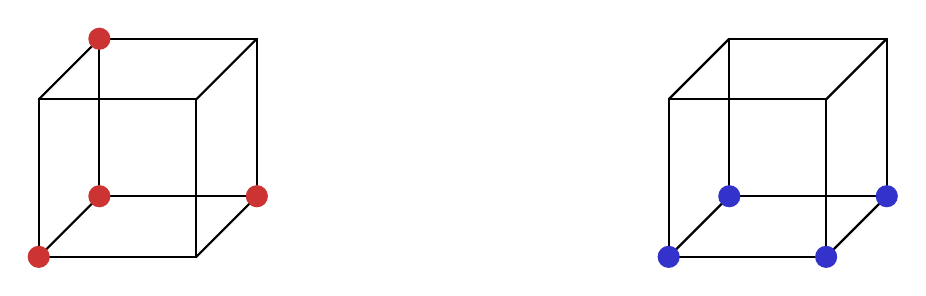
\begin{tikzpicture}

% Define colors for highlighting
\definecolor{highlight1}{rgb}{0.8,0.2,0.2}
\definecolor{highlight2}{rgb}{0.2,0.2,0.8}

% Cube on the left
\begin{scope}[xshift=-4cm, scale = 2]
  % Define vertices of the left cube
  \coordinate (A) at (0,0,0);
  \coordinate (B) at (1,0,0);
  \coordinate (C) at (1,1,0);
  \coordinate (D) at (0,1,0);
  \coordinate (E) at (0,0,1);
  \coordinate (F) at (1,0,1);
  \coordinate (G) at (1,1,1);
  \coordinate (H) at (0,1,1);

  % Draw edges of the left cube
  \draw[thick] (A) -- (B) -- (C) -- (D) -- cycle; % Bottom face
  \draw[thick] (E) -- (F) -- (G) -- (H) -- cycle; % Top face
  \draw[thick] (A) -- (E);
  \draw[thick] (B) -- (F);
  \draw[thick] (C) -- (G);
  \draw[thick] (D) -- (H);

  % Highlight chosen vertex and adjacent vertices
  \fill[highlight1] (A) circle (2pt); % Highlight vertex A
  \fill[highlight1] (B) circle (2pt); % Adjacent vertex to A
  \fill[highlight1] (D) circle (2pt); % Adjacent vertex to A
  \fill[highlight1] (E) circle (2pt); % Adjacent vertex to A
\end{scope}

% Cube on the right
\begin{scope}[xshift=4cm, scale = 2]
  % Define vertices of the right cube
  \coordinate (A') at (0,0,0);
  \coordinate (B') at (1,0,0);
  \coordinate (C') at (1,1,0);
  \coordinate (D') at (0,1,0);
  \coordinate (E') at (0,0,1);
  \coordinate (F') at (1,0,1);
  \coordinate (G') at (1,1,1);
  \coordinate (H') at (0,1,1);

  % Draw edges of the right cube
  \draw[thick] (A') -- (B') -- (C') -- (D') -- cycle; % Bottom face
  \draw[thick] (E') -- (F') -- (G') -- (H') -- cycle; % Top face
  \draw[thick] (A') -- (E');
  \draw[thick] (B') -- (F');
  \draw[thick] (C') -- (G');
  \draw[thick] (D') -- (H');

  % Highlight vertices on the lower face
  \fill[highlight2] (A') circle (2pt); % Lower face vertex
  \fill[highlight2] (B') circle (2pt); % Lower face vertex
  \fill[highlight2] (E') circle (2pt); % Lower face vertex
  \fill[highlight2] (F') circle (2pt); % Lower face vertex
\end{scope}
\end{tikzpicture}
\end{center}

A good guess is that balls are the best, i.e. sets of the form
\[
B(\emptyset, r) = X^{(\leq r)} = X^{(0)} \cup X^{(1)} \cup \cdots \cup X^{(r)}.
\]
What if the size of our set is between two levels, i.e. $|X^{(\leq r)}| \leq |A| \leq |X^{(\leq r + 1)}|$?

Our guess is to take $A$ with $X^{(\leq r)} \leq A \leq X^{(\leq r + 1)}$. If $A = X^{(\leq r)} \cup B$, where $B \subseteq X^{(r + 1)}$, then
\[
B(A) = (X^{(r+1)} - B) \cup \partial^{+}(B).
\]
So we would take $B$ to be an initial segment of lex, by Kruskal-Katona.

In the \emph{simplicial ordering}\index{simplicial ordering} of $\mathcal{P}(X)$, we set $x < y$ if either $|x| < |y|$, or $|x| = |y|$, but $x < y$ in lex.

Our aim is to show that initial segments of the simplicial ordering minimize the boundary. We do it by compression, in the spirit of KK.

Fix $A \subset \mathcal{P}(X)$. For $1 \leq i \leq n$, the \emph{$i$-selection}\index{$i$-selection} of $A$ are the families $A_-^{(i)}$, $A_+^{(i)} \subseteq \mathcal{P}(X - i)$ given by
\begin{align*}
	A_{-}^{(i)} &= \{x \in A \mid i \not \in x\}, \\
	A_{+}^{(i)} &= \{x-i \mid x \in A, i \in x\}.
\end{align*}
The \emph{$i$-compression}\index{$i$-compression} of $A$ is the family $C_i(A) \subseteq \mathcal{P}(X)$ given by, $(C_i(A))^{(i)}_{-}$ is the first $|A_{-}^{(i)}|$ elements of the simplicial ordering of $\mathcal{P}(X - i)$, and $(C_i(A))_{+}^{(i)}$ be the first $|A_{+}^{(i)}|$ elements of the simplicial ordering on $\mathcal{P}(X - i)$.

This is essentially doing a compression on each of the two $i$-level sub-hypercubes simultaneously.

A subset is \emph{$i$-compressed} if $C_i(A) = A$. Here a \emph{Hamming ball}\index{Hamming ball} is a family with $X^{(\leq r)} \subseteq A \subseteq X^{(\leq r + 1)}$ for some $r$.

\begin{theorem}[Harper's Theorem]
	Let $A \subseteq Q_n$, and let $C$ be the initial segment of the simplicial order with $|C| = |A|$. Then $|N(A)| \geq |N(C)|$. In particular, if
	\[
	|A| = \sum_{i = 0}^{k} \binom ni \implies |N(A)| \geq \sum_{i = 0}^{k + 1} \binom ni.
	\]
\end{theorem}

\begin{remark}
	\begin{enumerate}
		\item[]
		\item If we knew $A$ was a Hamming ball, we would be done by KK.
		\item Conversely, this theorem implies KK, as we could take $B \subseteq X^{(r)}$, and then apply theorem 1 to $A = X^{(\leq r - 1)} \cup B$.
	\end{enumerate}
\end{remark}

\begin{proofbox}
	We proceed by induction on $n$. For $n = 1$, this is trivial.

	Now suppose we are given $n > 1$, $A \subseteq Q_n$, and $1 \leq i \leq n$. Then we claim that
	\[
	|N(C_i(A))| \leq |N(A)|.
	\]
	Write $B$ for $C_i(A)$. Then we have
	\begin{align*}
		N(A)_{-} &= N(A_{-}) \cup A_+, \\
		N(A)_+ &= N(A_+) \cup A_-,
	\end{align*}
	and of course
	\begin{align*}
		N(B)_- &= N(B_-) \cup B_+, \\
		N(B)_+ &= N(B_+) \cup B_-.
	\end{align*}
	Now, $|B_+| = |A_+|$, and $|N(B_-)| \leq |N(A_-)|$ by induction. But $B_+$ is an initial segment of the simplicial ordering, and $N(B_-)$ is as well, as a neighbourhood of an initial segment is an initial segment.

	So, $B_+$ and $N(B_-)$ are nested. Hence $|N(B)_-| \leq |N(A)_-|$. Similarly, $|N(B)_+| \leq |N(A)_+|$, giving $|N(B)| \leq |N(A)|$.
% lecture 8
	Define a sequence $A_0, A_1, \ldots \subseteq Q_n$ as follows: Set $A_0 = A$, and having chose $A_0, \ldots, A_k$, if $A_k$ is $i$-compressed for all $i$, then stop the sequence with $A_k$.

	If not, pick $i$ with $C_i(A_k) \neq A_k$, and set $A_{k+1} = C_i(A_k)$, and continue. This must terminate, because the sum of the position of $x$ in the simplicial order, over all $x \in A_k$, is strictly decreasing.

	The final family $B = A_k$ satisfies $|B| = |A|$, and $|N(B)| \leq |N(A)|$, and is $i$-compressed for all $i$. 
\end{proofbox}

Does $B$ being $i$-compressed for all $i$ imply $B$ is an initial segment? No; consider a copy of $Q_2$ in $Q_3$. However,

\begin{lemma}
	Let $B \subseteq Q_n$ be $i$-compressed for all $i$, but not an initial segment of the simplicial order. Then either:
	\begin{itemize}
		\item $n$ is odd, say $n = 2k + 1$, and $B = X^{(\leq k)} - \{k+2, k+3, \ldots, 2k+1\} \cup \{1, 2, \ldots, k+1\}$,
	\item $n$ is even, say $n = 2k$, and $B = X^{(\leq k)} - \{1, k+2, \ldots, 2k\} \cup \{2, 3, \ldots, k+1\}$.
	\end{itemize}
\end{lemma}

Then we are done, as in each case $|N(B)| \geq |N(C)|$.

\begin{proofbox}
	Suppose that $B$ is not an initial segment of the simplicial ordering, so there is $x < y$ in the simplicial ordering with $x\not \in B$, $y \in B$.

	For each $1 \leq i \leq n$, we cannot have $i \in x$ and $i \in y$, since $B$ is $i$-compressed, and we also cannot have $i \not \in x$, $i \not \in y$ for the same reason.

	So $x = y^{c}$. Thus for each $y \in B$, there is at most one earlier $x$ with $x \not \in B$, namely $x = y^{c}$, and for each $x \not \in B$, there is at most one later $y$ with $y \in B$, namely $y = x^{c}$.

	So $B = \{z \mid z \leq y\} - \{x\}$, with $x$ the predecessor of $y$, and $x = y^{c}$. Hence if $n = 2k+1$, then $x$ must be the last $k$-set, and if $n = 2k$ then $x$ is the last $k$-set with $1$.
\end{proofbox}

This completes the proof of Harper's theorem.

\begin{remark}
	\begin{enumerate}
		\item[]
		\item We can also prove Harper's theorem using $UV$-compressions.
		\item We can also prove KK using $i$-compressions.
	\end{enumerate}
\end{remark}

For $A \subseteq Q_n$ and $t = 1, 2, 3, \ldots$, the $t$-neighbourhood of $A$ is
\[
	A_{(t)} = N^{t}(A) = \{x \in Q_n \mid d(x, A) \leq t\}.
\]

\begin{corollary}
	Let $A \subseteq Q_n$ with
	\[
	|A| \geq \sum_{i = 0}^r \binom ni.
	\]
	Then for all $t \leq n - r$,
	\[
	|A_{(t)}| \geq \sum_{i = 0}^{r + t} \binom ni.
	\]
\end{corollary}

\begin{proofbox}
	Use Harper's theorem and induction (the neighbourhood of an initial segment of simplicial is another initial segment).
\end{proofbox}

To get a feeling for the strength of the corollary, we will need some estimates on the size of things like
\[
\sum_{i = 0}^{r} \binom ni
\]

\begin{proposition}
	Let $0 < \eps < 1/4$. Then,
	\[
	\sum_{i = 0}^{\lfloor (\frac{1}{2} - \eps) n \rfloor} \binom ni \leq \frac{1}{\eps} e^{-\eps^2 n/t} 2^{n}.
	\]
\end{proposition}

\begin{proofbox}
	For $i \leq \lfloor (\frac{1}{2} - \eps) n \rfloor$, we have
	\[
		\frac{\binom n{i-1}}{\binom ni} = \frac{i}{n - i + 1} \leq \frac{(\frac{1}{2} - \eps) n}{(\frac{1}{2} + \eps)n} = \frac{\frac{1}{2} - \eps}{\frac{1}{2} + \eps} = 1 - \frac{2 \eps}{\frac{1}{2} + \eps} \leq 1 - 2 \eps.
	\]
	Hence, summing this as a GP,
	\[
		\sum_{i = 0}^{\lfloor ( \frac{1}{2} - \eps) n \rfloor} \binom ni \leq \frac{1}{2 \eps} \binom n{\lfloor ( \frac{1}{2} - \eps) n \rfloor}.
	\]
	The same argument tells us that
	\[
		\binom{n}{\lfloor (\frac{1}{2} - \eps) n \rfloor} \leq \binom{n}{\lfloor ( \frac{1}{2} - \frac{\eps}{2}) n \rfloor} (1 - \eps)^{\frac{\eps n}{2} - 1} \leq 2^{n} \cdot 2 (1 - \eps)^{\eps n / 2} \leq 2^{n} \cdot 2 e^{-\eps^2 n/2}.
	\]
	Thus we get
	\[
	\sum_{i = 0}^{\lfloor (\frac{1}{2} - \eps) n \rfloor} \binom ni \leq \frac{1}{2 \eps} 2 e^{-\eps^2n / 2} 2^{n}.
	\]
\end{proofbox}

% lecture 9

\begin{theorem}
	Let $0 < \eps < 1/4$, $A \subseteq Q_n$. Then
	\[
		\frac{|A|}{2^{n}} \geq \frac{1}{2} \implies \frac{|A_{(\eps n)}|}{2^{n}} \geq 1 - \frac{2}{\eps} e^{-\eps^2n/2}.
	\]
\end{theorem}

In other words, half-sized sets have exponentially large $\eps n$-neighbourhoods.

\begin{proofbox}
	It is enough to show that if $\eps n$ is an integer, then
	\[
	\frac{|A_{(\eps n)|}}{2^{n}} \geq 1 - \frac{1}{\eps} e^{-\eps^2n/2}.
	\]
	We have that
	\[
	|A| \geq \sum_{i = 0}^{\lceil n/2 - 1 \rceil} \binom ni,
	\]
	so by Harper, we have
	\[
	|A_{(\eps n)}| \geq \sum_{i = 0}^{\lceil n/2 - 1 + \eps n\rceil} \binom ni.
	\]
	So
	\[
	|A_{(\eps n)}^{c}| \leq \sum_{\lceil n/2 + \eps n \rceil}^n \binom ni = \sum_{i = 0}^{\lfloor n/2 - \eps n \rfloor} \binom ni \leq \frac{1}{\eps} e^{-\eps^2n/2} \cdot 2^{n}.
	\]
\end{proofbox}

\begin{remark}
	The same would show that, for small sets,
	\[
	\frac{|A|}{2^{n}} \geq \frac{2}{\eps} e^{-\eps^2n/2} \implies \frac{|A_{(2 \eps n)}|}{2^{n}} \geq 1 - \frac{2}{\eps} e^{-\eps^2n/2}.
	\]
\end{remark}

\subsection{Concentration of Measure}%
\label{sub:conc_m}

Say $f : Q_n \to \mathbb{R}$ is \emph{Lipschitz}\index{Lipschitz} if $|f(x) - f(y)| \leq 1$ for all $x, y$ adjacent. For $f : Q_n \to \mathbb{R}$, say $M \in \mathbb{R}$ is a \emph{L\'evy mean}\index{L\'evy mean} or the \emph{median}\index{median} of $f$ if
\[
	|\{x \in Q_n \mid f(x) \leq M\}| \leq 2^{n-1} \qquad \text{and} \qquad |\{x \in Q_n \mid f(x) \geq M\}| \geq 2^{n-1}.
\]

We are now ready to show that every well-behaved function on the cube $Q_n$ is roughly constant nearly everywhere.

\begin{theorem}
	Let $f: Q_n \to \mathbb{R}$ be Lipschitz with median $M$. Then,
	\[
		\frac{|\{x \mid |f(x) - M| \leq \eps n\}|}{2^{n}} \geq 1 - \frac{4}{\eps} e^{-\eps^2n/2},
	\]
	for any $0 < \eps < 1/4$.
\end{theorem}

Note that this is the concentration of measure phenomenon.

\begin{proofbox}
	Let $A = \{x \mid f(x) \leq M\}$. Then
	\[
	\frac{|A|}{2^{n}} \geq \frac{1}{2} \implies \frac{|A_{(\eps n)|}}{2^{n}} \geq 1 - \frac{2}{\eps} e^{-\eps^2n/2}.
	\]
	But $f$ is Lipschitz, so if $x \in A_{(\eps n)}$, then $f(x) \leq M + \eps n$. Then,
	\[
		\frac{|\{x \mid f(x) \leq M + \eps n\}|}{2^{n}} \geq 1 - \frac{2}{\eps} e^{-\eps^2n/2}.
	\]
	Similarly,
	\[
		\frac{|\{x \mid f(x) \geq M - \eps n\}|}{2^{n}} \geq 1 - \frac{2}{\eps} e^{-\eps^2n/2}.
	\]
	Putting this together,
	\[
		\frac{|\{x \mid |f(x) - M| \leq \eps n\}|}{2^{n}} \geq 1 - \frac{4}{\eps} e^{-\eps^2n/2},
	\]
\end{proofbox}

Let $G$ be a graph of diameter $D$. Write
\[
\alpha(G, \eps) = \max \left\{ 1 - \frac{|A_{(\eps D)}|}{|G|} \bigm| A \subseteq G, \frac{|A|}{|G|} \geq \frac{1}{2} \right\}.
\]
So $\alpha(G, \eps)$ says that half-sized sets have larger $\eps D$-neighbourhoods.

We say that a sequence of graphs is a \emph{L\'evy family}\index{L\'evy family} if $\alpha(G_n, \eps) \to 0$ as $n \to \infty$, for each $\eps > 0$.

This theorem tells us that the sequence $(Q_n)$ is a L\'evy family, and it is even a \emph{normal L\'evy family}\index{normal L\'evy family}, meaning that $\alpha(G_n, \eps)$ is exponentially small in $n$, for each $\eps > 0$.

For any L\'evy family we have concentration of measure. Most naturally occurring families of graphs are L\'evy families, for example $(S_n)$ where $S_n$ is made into a graph by joining permutations joined by a transposition.

We can also define $\alpha(X, \eps)$ similarly for an metric measure space $X$, of finite measure and finite diameter.

\begin{exbox}
	$(S^{n})$ is a L\'evy family. This requires two ingredients.
	\begin{enumerate}
		\item An isoperimetric inequality on $S_n$: for $A \subseteq S_n$ and $C$ a circular cap with $|C| = |A|$, we have $|A_{(\eps})| \geq |C_{(\eps)}|$.

			This is proven by compression; consider laying the sphere out on some way, and then vertically projecting each point if possible. This is known as two-point symmetrisation.
		\item Then we estimate the size. A circular cap of measure $1/2$ is the cap of angle $\pi/2$. Then $C_{(\eps)}$ is the circular cap of angle $\pi/2 + \eps$. This has measure about
			\[
			\int_\eps^{\pi/2} \cos^{n-1}t \diff t \to 0.
			\]
	\end{enumerate}
	Moreover this is a normal L\'evy family.
\end{exbox}

We have deduced concentration of measure from an isoperimetric family. Conversely,

\begin{proposition}
	Let $G$ be a graph such that for any Lipschitz function $f : G  \to \mathbb{R}$ with median $M$, we have
	\[
		\frac{|\{x \in G \mid |f(x) - M| > t\}}{|G|} \leq \alpha
	\]
	for some given $t, \alpha$. Then for all $A \in G$, if $\frac{|A|}{|G|} \geq \frac{1}{2}$, we have
	\[
	\frac{|A_{(t)}|}{|G|} \geq 1 - \alpha.
	\]
\end{proposition}

\begin{proofbox}
	The function $f(x) = d(x, A)$ is Lipschitz, and has $0$ as its median since at least half of the values take $0$. So
	\[
		\frac{|\{x \in G \mid x \not \in A_{(t)}\}|}{|G|} \leq \alpha.
	\]
\end{proofbox}

% lecture 10

\subsection{Edge-isoperimetric Inequalities}%
\label{sub:eip}

For a subset $A$ of vertices of a graph $G$, the \emph{edge-boundary}\index{edge-boundary} of $A$ is
\[
\partial_e A = \partial A = \{xy \in G \mid x \in A, y\notin A\}.
\]
An inequality of the form $|\partial A| \geq f(|A|)$ for all $A \subseteq G$ is an \emph{edge-isoperimetric inequality}\index{edge-isoperimetric inequality} on $G$.

What happens in $Q_n$? Given $|A|$, which $A \subseteq Q_n$ could we take to maximize $|\partial A|$? For example, if $|A| = 4$, then the 

\begin{center}
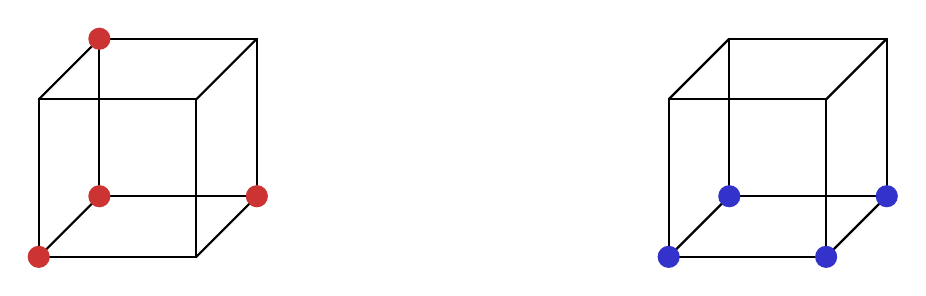
\begin{tikzpicture}

% Define colors for highlighting
\definecolor{highlight1}{rgb}{0.8,0.2,0.2}
\definecolor{highlight2}{rgb}{0.2,0.2,0.8}

% Cube on the left
\begin{scope}[xshift=-4cm, scale = 2]
  % Define vertices of the left cube
  \coordinate (A) at (0,0,0);
  \coordinate (B) at (1,0,0);
  \coordinate (C) at (1,1,0);
  \coordinate (D) at (0,1,0);
  \coordinate (E) at (0,0,1);
  \coordinate (F) at (1,0,1);
  \coordinate (G) at (1,1,1);
  \coordinate (H) at (0,1,1);

  % Draw edges of the left cube
  \draw[thick] (A) -- (B) -- (C) -- (D) -- cycle; % Bottom face
  \draw[thick] (E) -- (F) -- (G) -- (H) -- cycle; % Top face
  \draw[thick] (A) -- (E);
  \draw[thick] (B) -- (F);
  \draw[thick] (C) -- (G);
  \draw[thick] (D) -- (H);

  % Highlight chosen vertex and adjacent vertices
  \fill[highlight1] (A) circle (2pt); % Highlight vertex A
  \fill[highlight1] (B) circle (2pt); % Adjacent vertex to A
  \fill[highlight1] (D) circle (2pt); % Adjacent vertex to A
  \fill[highlight1] (E) circle (2pt); % Adjacent vertex to A
\end{scope}

% Cube on the right
\begin{scope}[xshift=4cm, scale = 2]
  % Define vertices of the right cube
  \coordinate (A') at (0,0,0);
  \coordinate (B') at (1,0,0);
  \coordinate (C') at (1,1,0);
  \coordinate (D') at (0,1,0);
  \coordinate (E') at (0,0,1);
  \coordinate (F') at (1,0,1);
  \coordinate (G') at (1,1,1);
  \coordinate (H') at (0,1,1);

  % Draw edges of the right cube
  \draw[thick] (A') -- (B') -- (C') -- (D') -- cycle; % Bottom face
  \draw[thick] (E') -- (F') -- (G') -- (H') -- cycle; % Top face
  \draw[thick] (A') -- (E');
  \draw[thick] (B') -- (F');
  \draw[thick] (C') -- (G');
  \draw[thick] (D') -- (H');

  % Highlight vertices on the lower face
  \fill[highlight2] (A') circle (2pt); % Lower face vertex
  \fill[highlight2] (B') circle (2pt); % Lower face vertex
  \fill[highlight2] (E') circle (2pt); % Lower face vertex
  \fill[highlight2] (F') circle (2pt); % Lower face vertex
\end{scope}
\end{tikzpicture}
\end{center}

It follows that maybe subcubes are the best. What if we have $A \subseteq Q_n$ with $2^{k} < |A| < 2^{k+1}$? Then we should take $A = \mathcal{P}([k])$ along with some sets in $\mathcal{P}([k+1])$.

So we define the following ordering: for $x, y \in Q_n$ and $x \neq y$, we say that $x < y$ in the \emph{binary ordering}\index{binary ordering} on $Q_n$ if $\max x \triangle y \leq y$. Equivalently,
\[
x < y \iff \sum_{i \in x} 2^{i} < \sum_{i \in y} 2^{i}.
\]
For example in $Q_3$, the sets are ordered
\[
\emptyset, 1, 2, 12, 3, 13, 23, 123.
\]
For $A \subseteq Q_n$ and $1 \leq i \leq n$, we define the \emph{$i$-binary-compression}\index{binary compression} $B_i(A) \subseteq Q_n$ by giving it $i$-sections:
\begin{align*}
(B_i(A))^{(i)}_- &= \text{initial segment of binary on } \mathcal{P}(X - i) \text{ of size } |A_-^{(i)}|, \\
(B_i(A))^{(i)}_+ &= \text{initial segment of binary on } \mathcal{P}(X - i) \text{ of size } |A_+^{(i)}|.
\end{align*}
So $|B_i(A)| |A|$. We say that $A$ is \emph{$i$-binary-compressed} if $B_i(A) = A$.

\begin{theorem}[Edge-isoperimetric Inequality in $Q_n$]
	Let $A \subseteq Q_n$ and $C$ be the initial segment of binary on $Q_n$ with $|C| = |A|$. Then $|\partial C| \leq |\partial A|$. In particular, if $|A| = 2^{k}$, then $|\partial A| \geq 2^{k}(n-k)$.
\end{theorem}

\begin{remark}
	This is sometimes called the theorem of Harper, Lindsey, Bernstein and Hart.
\end{remark}

\begin{proofbox}
	We proceed by induction on $n$. $n = 1$ is trivial.

	For $n > 1$, $A \subseteq Q_n$, $1 \leq i \leq n$, we claim that $|\partial B_i(A)| \leq |\partial A|$.

	Indeed, write $B$ for $B_i(A)$. Then
	\begin{align*}
		|\partial A| &= |\partial(A_-)| + |\partial(A_+)| + |A_+ \triangle A_-|, \\
		|\partial B| &= |\partial(B_-)| + |\partial(B_+)| + |B_+ \triangle B_-|.
	\end{align*}
	By induction, $|\partial(B_-)| \leq |\partial(A_-)|$ and $|\partial(B_+)| \leq |\partial(A_+)|$. Also, the set $B_+$ and $B_-$ are nested, as each is an initial segment of binary on $\mathcal{P}(X - i)$.

	Therefore, certainly we have $|B_+ \triangle B_-| \leq |A_+ \triangle A_-|$. So $|\partial B| \leq |\partial A|$.

	Define a sequence $A_0, A_1, \ldots \subseteq Q_n$ as follows. Set $A_0 = A$. Having defined $A_0, \ldots, A_k$, if $A_k$ is $i$-binary-compressed for all $i$, then stop the sequence. If not, choose $i$ with $B_i(A_k) \neq A_k$, and put $A_{k+1} = B_i(A_k)$.

	This must terminate as the function
	\[
		k \mapsto \sum_{x \in A_k} (\text{position of $x$ in binary})
	\]
	is strictly decreasing. Now the final family $B = A_k$ satisfies $|B| = |A|$ and $|\partial B| \leq |\partial A|$.
\end{proofbox}

Note that $B$ need not be an initial segment of binary, for example take $\{\emptyset, 1, 2, 3\} \subseteq Q_3$. However these are the only counterexamples.

\begin{lemma}
	Let $B \subseteq Q_n$ be binary compressed for all $i$, that is not an initial segment of binary. Then
	\[
		B = \mathcal{P}(n - 1) - \{12 \ldots n-1\} \cup \{n\}.
	\]
\end{lemma}

Then we are done, as clearly $|\partial B| \geq |\partial C|$, since $C = \mathcal{P}(n-1)$.

\begin{proofbox}
	As $B$ is not an initial segment there exists $x < y$ with $x \not \in B$, $y \in B$.

	Thus for all $i$, we cannot have $i \in x, y$ or $i \notin x, y$, as $B$ is $i$-binary-compressed. So $y = x^{c}$.

	Thus for each $y \in B$, there is at most one earlier $x \in B$, and for each $x \not \in B$ there is at most one later $y \in B$. So $B = \{z \mid z \leq y\} - \{x\}$, where $y$ is the predecessor of $y$ and $y = x^{c}$.

	So we must have $y = \{n\}$.
\end{proofbox}

This concludes the proof of theorem 2.4.

% lecture 11

\begin{remark}
	It is vital in this proof, and the proof of Harper's that the extremal sets were nested.
\end{remark}

The \emph{isoperimetric number}\index{isoperimetric number} of a graph  $G$ is
\[
	i(G) = \min \left\{ \frac{|\partial A|}{|A|} \mid A \subseteq G, \frac{|A|}{|G|} \leq \frac{1}{2} \right\}.
\]

\begin{corollary}
	$i(Q_n) = 1$.
\end{corollary}

\begin{proofbox}
	Taking $A = \mathcal{P}(n-1)$, we get that $i(Q_n) \leq 1$ (every edge is between $x$ and $x + n$).

	To show that $i(Q_n) \geq 1$, we need to show that if $C$ is an initial segment of binary with $|C| \leq 2^{n-1}$, then $|\partial C| \geq |C|$. But $C \subseteq \mathcal{P}(n-1)$, so certainly $|\partial C| \geq |C|$.
\end{proofbox}

\subsection{Inequalities in the Grid}%
\label{sub:ineq_gid}

For any $k = 2, 3, \ldots$,  the \emph{grid}\index{grid} is the graph on $[k]^{n}$ in which $x$ is joined to $y$ if for some $i$, we have $x_j = y_j$ for $j \neq i$, and $|x_i - y_i| = 1$.

For example, we can draw the 4 grid.

Note that for $k = 2$, this is exactly $Q_n$. Do we have analogues of Sperner's and KK for the grid? We start with the vertex-isoperimetric problem; which sets $A \subseteq [k]^{n}$ (of a given size) minimise $|N(A)|$?

In $[k]^2$, we can either consider a diagonal or a square. The diagonal cut seems to be better.

This suggests that we go up in levels according to
\[
|x| = \sum_{i = 1}^n |x_i|,
\]
i.e. we take $\{x \in [k]^{n} \mid |x| \leq r\}$. What if
\[
|\{x \in [k]^{n} \mid |x| \leq r\}| < |A| < |\{x \in [k]^{n} \mid |x| \leq r+1\}|?
\]
In this case, we take $A = \{x \in [k]^{n} \mid |x| \leq r\}$, and some point with $|x| = r + 1$. The points we pick should be those which keep $x_1$ large.

This suggests in the \emph{simplicial ordering}\index{simplicial ordering} on $[k]^{n}$, we set $x < y$ if either $|x| < |y|$ or $|x| = |y|$ and $x_i > y_i$ where $i$ is the minimal element where they differ.

\begin{exbox}
	On $[3]^2$, the ordering is
	\[
		(1,1), (2, 1), (1, 2), (3, 1), (2, 2), (1, 3), (3, 2), (2, 3), (3, 3).
	\]
	On $[4]^{3}$, the ordering is
	\begin{align*}
		(1, 1, 1), &(2, 1, 1), (1, 2, 1), (1, 1, 2), (3, 1, 1), (2, 2, 1), (2, 1, 2), (1, 3, 1), \\
			   &(1, 2, 2), (1, 1, 3), (4, 1, 1), (3, 2, 1), \ldots
	\end{align*}
\end{exbox}

For $A \subseteq [k]^{n}$ for some $k \geq 2$ and $1 \leq i \leq n$, the \emph{$i$-sections}\index{$i$-sections} of $A$ are the sets $A_1, \ldots, A_k \subseteq [k]^{n-1}$ defined by
\[
A_t = A_t^{(i)} = \{x \in [k]^{n-1} \mid (x_1, x_2, \ldots, x_{i-1}, t, x_i, x_{i+1}, \ldots, x_{n-1}) \in A \}.
\]
The \emph{$i$-compression}\index{$i$-compression} of $A$ is $C_i(A) \subseteq [k]^{n}$ defined by giving its $i$-sections:
\[
	C_i(A) = \text{initial segment of $[k]^{n-1}$ of size } |A_t|.
\]
Essentially, we are going layer by layer in the $i$'th direction, and shoving everything into an initial segment of simplicial.

\begin{theorem}[Vertex-Isoperimetric Inequality in the Grid]
	Let $A \subseteq [k]^{n}$, and let $C$ be the initial segment of simplicial of $[k]^{n}$ with $|C| = |A|$. 

	Then $|N(C)| \leq |N(A)|$. In particular, if $|A| \geq |\{x \mid |x| \leq r\}$, then $|N(A)| \geq |\{x \mid |x| \leq r+1\}$.
\end{theorem}

\begin{proofbox}
	We proceed by induction on $n$. $n = 1$ is trivial, if $A \subseteq [k]^{1} \neq \emptyset$, then $|N(A)| \geq |A| + 1 = |N(C)|$.

	Given $n > 1$ and $A = [k]^{n}$, fix $1 \leq i \leq n$. We claim that $|N(C_i(A))| \leq |N(A)|$.

	Indeed, write $B$ for $C_i(A)$. For any $1 \leq t \leq k$, we have
	\[
	N(A)_t = N(A_t) \cup A_{t-1} \cup A_{t+1},
	\]
	and similarly $N(B)_t = N(B_t) \cup B_{t-1} \cup B_{t+1}$. Now $|B_{t-1}| = |A_{t-1}|$, and $|B_{t+1}| = |A_{t+1}|$, and $|N(B_t)| \leq |N(A_t)|$, by the induction hypothesis. But the sets $B_{t-1}, B_{t+1}$ and $N(B_t)$ are nested as each is an initial segment of simplicial on $[k]^{n-1}$.

	Hence $|N(B)_t| \leq |N(A)_t|$, so $|N(B)| \leq |N(A)|$.

	Among all $B \subseteq [k]^{n}$ with $|B| = |A|$ and $|N(B)| \leq |N(A)|$, pick one with sum of simplicial positionings the smallest. Then $B$ is $i$-compressed for all $i$.

	We are very far from being done. To continue, we split into two cases.

	Case 1: $n = 2$. What we know is precisely that $B$ is a down-set.
% lecture 12
	Let $r = \min\{|x| \mid x \not \in B\}$, and $s = \max\{|x| \mid x \in B\}$. We may assume that $r \leq s$, since if $r = s + 1$, then $B = \{x \mid |x| \leq s\}$, hence $B = C$.

	If $r = s$, then
	\[
		\{x \mid |x| \leq r - 1\} \subseteq B \subseteq \{x \mid |x| \leq r\},
	\]
	so clearly $|N(B)| \geq |N(C)|$.

	If  $r < s$, then we cannot have $\{x \mid |x| = s\} \subseteq B$, because then also $\{x \mid |x| = r\} \subseteq B$ as $B$ is a down set.

	So there is $y, y'$ with $|y| = |y'| = s$, $y \in B$ and $y' \not \in B$, and $y' = y \pm (e_1 - e_2)$, by DIVT.

	Similarly, we cannot have $\{x \mid |x| = r\} \cap B = \emptyset$, otherwise $\{x \mid |x| = s\} \cap B = \emptyset$, again as $B$ is a down set. So there is $x, x'$ with $|x| = |x'| = r$, $x \not \in B$, $x' \in B$ and $x' = x \pm (e_1 - e_2)$.

	Now let $B' = B \cup \{x\} - \{y\}$. From $B$ we lost at least one point in the neighbourhood, namely $y + e_1$ or $y + e_2$, and gained at most one point, so $|N(B')| \leq |N(B)|$. This contradicts the minimality of $B$.

	Case 2: $n \geq 3$. For any $1 \leq i \leq n-1$ and any $x \in B$ with $x_n > 1$ and $x_i < k$, we must have that
	\[
	x - e_n + e_i \in B,
	\]
	as $B$ is $j$-compressed, for any $j \neq 1, n$.

	So, considering the $n$-sections of $B$, we have that $N(B_t) \subseteq B_{t-1}$ for all $t = 2, \ldots, k$. Recall that $N(B)_t = N(B_t) \cup B_{t+1} \cup B_{t-1}$, so in fact $N(B)_t = B_{t-1}$. Thus,
	\[
	|N(B)| = |B_{k-1}| + |B_{k-2}| + \cdots + |B_1| + |N(B_1)| = |B| - |B_k| + |N(B_1)|.
	\]
	Similarly, $|N(C)| = |C| - |C_k| + |N(C_1)|$. So to show $|N(C)| \leq |N(B)|$, it is enough to show that $|B_k| \leq |C_k|$, and $|B_1| \geq |C_1|$, since $|N(C_1)|$ is minimal for its size.

	To show $|B_k| \leq |C_k|$, define a set $D \subseteq [k]^{n}$  as follows: put $D_k = B_k$, and for $t = k-1, k-2, \ldots, 1$ set $D_t = N(D_{t-1})$.

	Then $D \subseteq B$ so $|D| \leq |B|$, and in fact $D$ is an initial segment of simplicial so $D \subseteq C$, showing $|B_k| = |D_k| \leq |C_k|$.

	To show $|B_1| \geq |C_1|$, define a set $E \subseteq [k]^{n}$ as follows: put $E_1 = B_1$, and for $t = 2, 3, \ldots, k$ set $E_t = \{x \in [k]^{n-1} \mid N(\{x\}) \subseteq E_{t-1}\}$.

	Then $E \supseteq B$ so $|E| \supseteq |B|$ and $E$ is an initial segment of simplicial, so $E \supseteq C$, whence $|B_1| = |E_1| \geq |C_1|$.

	This shows the theorem.
\end{proofbox}

\begin{corollary}
	Let $A \subseteq [k]^{n}$ with $|A| \geq |\{x \mid |x| \leq r\}|$. Then $|A_{(t)}| \geq |\{x \mid |x| \leq r + t\}|$.
\end{corollary}

\begin{remark}
	We can check from the corollary that for $k$ fixed, the sequence $([k]^{n})$ is a L\'evy family.
\end{remark}

We now look at the edge-isoperimetric inequality in the grid. Which set $A \subseteq [k]^{n}$ should we take to minimize $|\partial A|$? For example, in $[k]^2$, we can look at squares and triangles, which suggest that squares are the best.

However, there are nasty things that happen as we grow the size of of $|A|$. When $|A|$ is 1/4 of the total size of $[k]^2$, the square does equally as well as the column, and for greater sizes columns do better.

A similar thing occurs at $3/4$ of the total size, when the column equals a cosquare, and at large sizes the cosquare does the best. So we have phase transitions at $|A| = k^2/4$ and $3k^2/4$, when the extremal sets are not nested. This seems to rule out compression methods (insert image).

And in $[k]^3$, we have even more phase transitions:
\[
	[a]^3 \to [a]^2 \times [k] \to [a] \times [k]^2 \to ([a]^2 \times [k])^{c} \to ([a]^3]^{c}.
\]
Hence in $[k]^{n}$, up to halfway we get $n - 1$ of these phase transitions.

% lecture 13

Note that if $A = [a]^{d} \times [k]^{n-d}$, then $|\partial A| = d a^{d-1} k^{n-d} = d |A|^{1 - 1/d} k^{n/d - 1}$.

\begin{theorem}
	Assuming that $A \subseteq [k]^{n}$ and $|A| \leq k^{n}/2$, then
	\[
		|\partial A| \geq \min \{ d |A|^{1 - 1/d} k^{n/d - 1} \mid 1 \leq d\leq n \}.
	\]
\end{theorem}

This just says that some set of the form $[a]^{d} \times [k]^{n-d}$ is the best. The following is non-examinable.

\begin{proofbox}
	We give a sketch of the proof. The idea is induction on $n$: $n = 1$ is trivial.

	Take $A \subseteq [k]^{n}$, with $|A| \leq k^{n}/2$ and $n > 1$. Without loss of generality, assume that $A$ is a down-set, by compressing in each direction $1 \leq i \leq n$. For any $1 \leq i \leq n$, define $C_i(A)$ by defining its sections:
	\[
		C_i(A)_t = \text{extremal set of size } |A_t| \text{ in } [k]^{n-1}.
	\]
	This will be a set of the form $[a]^{d} \times [k]^{n - 1 - d}$, or a complement. Say $B = C_i(A)$. We want to say something like $|\partial B| \leq |\partial A|$. Since $A$ is a down set, we can write
	\[
	|\partial A| = |\partial A_1| + \cdots + |\partial A_k| + |A_1| - |A_k|,
	\]
	since the sections of $A$ are nested. But for $B$, we do not have the same expression, since it is not a down-set: extremal sets may not be nested. Indeed, we may have $|\partial B| > |\partial A|$, by choosing the sections of $A$ on opposite sides of a phase transition.

	The idea we have to solve this is to introduce a ``fake'' boundary $\partial'$, where $\partial' A \leq \partial A$ and $\partial' = \partial$ on extremal sets. Then we can try to show that $C_i$ decreases $\partial'$. Consider defining
	\[
	\partial' A = \sum_t |\partial A_t| + |A_1| - |A_k|,
	\]
	where $A_t$ is the $t$'th section in the $i$'th direction. Then $\partial' A \leq |\partial A|$ for all $A$, we have equality for extremal sets (as equality holds for down-sets), and $\partial' C_i(A) \leq \partial ' A$. However, for any $j \neq i$, $C_j(A)$ does not decrease the edge perimeter. One potential fix is trying
	\[
	\partial'' A = \sum_i (|A_1^{(i)}| - |A_k^{(i)}|).
	\]
	But this also fails, if we take e.g. $A$ to be the outer-shell of $[k]^{n}$. Collecting our results,
	\begin{align*}
		|\partial A| &\geq \partial ' A \geq \partial' B = \sum_t |\partial B_t| + |B_1| - |B_k| \\
			     &= \sum_t f(|B_t|) + |B_1| - |B_k|,
	\end{align*}
	where $f$ is the extremal function in $[k]^{n-1}$. Note that $f$ is the pointwise minimum of functions of the form $c x^{1- 1/d}$ and $c (k^{n-1} - x)^{1 - 1/d}$, which are concave. So $f$ is concave.

	Consider varying $|B_2|, \ldots, |B_{k-1}|$ while keeping $|B_2| + \cdots + |B_{k-1}|$ constant, and ensuring $|B_1| \geq |B_2| \geq \cdots \geq |B_{k-1}| \geq |B_k|$. To minimize this concave function, we should take
	\[
	C_t = 
	\begin{cases}
		B_1 & 1 \leq t \leq r, \\
		B_k & r+1 \leq t \leq k,
	\end{cases}
	\]
	for some $r$. Then we have
	\begin{align*}
		|\partial A| &= \partial' A \geq \partial' B \geq \partial C = r f(|B_1|) + (k - r) f(|B_k|) + |B_1| - |B_k|.
	\end{align*}
	But now $C$ is still not a down set. Now to improve this further, vary $|B_1|$ while keeping $r |B_1| + (k - r) |B_k|$ fixed (for fixed $r$), and $|B_1| \geq |B_k|$. This is concave in $|B_1|$, as it is a sum of concave functions. Hence we either make $|B_1|$ as big or as small as possible.

	If we let $D$ be this set, then $D$ must have one of the following forms:
	\begin{itemize}
		\item $|B_1| = |B_k|$, i.e. $D_t = D_1$ for all $t$.
		\item $|B_k| = 0$, so $D_t = D_1$ for all $t \leq r$, and $D_t = \emptyset$ for $t > r$.
		\item $B_1$ is maximal, so $D_t = [k]^{n-1}$ for $t \leq r$, and $D_t = D_k$ for $t > r$.
	\end{itemize}
	But finally, this $D$ has become a down-set. Hence
	\[
	|\partial A| = \partial' A \geq \partial' B \geq \partial' C \geq \partial' D = |\partial D|.
	\]
	So we can compress by going directly $A \to D$. This allows us to finish as before.
\end{proofbox}

\begin{remark}
	We were a bit sloppy as we assumed the sections $B_i$ were exactly of the form $[a]^{d} \times [k]^{n-d}$, however this may not be the case if $|B_i|$ is not of this form. To fix this, work instead in $[0, 1]^{n}$, and then take a discrete approximation.
\end{remark}

This concludes the non-examinable discussion.

% lecture 14

\begin{remark}
	Very few isoperimetric inequalities are known (even approximately). For example, take isoperimetric in a layer: in $X^{(r)}$, join two vertices $x, y$ if $|x \cap y| = r - 1$. This is open; the nicest special case if $r = n/2$, where it is conjectured that balls are the best, i.e. sets of the form
	\[
		\{x \in [2r]^{(r)} \mid |x \cap [r]| \geq t\}.
	\]
\end{remark}

\newpage

\section{Intersecting Families}%
\label{sec:if}

\subsection{\texorpdfstring{$t$}{t}-intersecting Families}%
\label{sub:tif}

$A \subseteq \mathcal{P}(X)$ is called \emph{$t$-intersecting}\index{$t$-intersecting} if $|x \cap y| \geq t$, for all $x, y \in A$. How large can a $t$-intersecting family be?

\begin{exbox}
Take $t = 2$. We could take $\{x \mid 1, 2 \in x\}$, which has size $1/4 \cdot 2^{n}$.

Or we could take $\{x \mid |x| \geq n/2 + 1\}$. This has size about $1/2 \cdot 2^{n}$.
\end{exbox}

\begin{theorem}[Katona's $t$-intersecting Theorem]
	Let $A \subseteq \mathcal{P}(X)$ be $t$-intersecting, where $n + t$ is event. Then
	\[
	|A| \leq \left| X^{(\geq \frac{n+t}{2})} \right|.
	\]
\end{theorem}

\begin{proofbox}
	For any $x, y \in A$, we have $|x \cap y| \geq t$, so $d(x, y^{c}) \geq t$. So writing $\bar A$ for $\{y^{c} \mid y \in A\}$, we have $d(A, \bar A) \geq t$, i.e. $A_{(t - 1)}$ is disjoint from $\bar A$.

	Suppose that $|A| \geq |X^{(\geq \frac{n+t}{2})}|$. Then by Harper,
	\[
	|A_{(t-1)}| \geq |X^{(\geq \frac{n+t}{2} - (t - 1)}| = |X^{(\geq \frac{n-t}{2} + 1)}|.
	\]
	But $A_{(t-1)}$ is disjoint from $\bar A$, which has size greater than $|X^{(\leq \frac{n-t}{2})}|$, contradicting $|A_{(t-1)}| + |\bar A|\leq 2^{n}$.
\end{proofbox}

What about $t$-intersecting families of $A \subseteq X^{(r)}$? We might guess that the best is
\[
	A_0 = \{x \in X^{(r)} \mid [t] \subseteq x\}.
\]
We could also try
\[
	A_\alpha = \{x \in X^{(r)} \mid |x \cap [t + 2\alpha]| \geq t + \alpha\},
\]
for $\alpha = 1, 2, \ldots, r - t$.
\begin{exbox}
	Take $2$-intersecting subsets of $[n]^{(4)}$.
	\begin{itemize}
		\item If $n = 7$, then $|A_0| = \binom 52 = 10$, $|A_1| = 1 + \binom 43 \binom 31 = 13$, $|A_2| = \binom 64 = 15$.
		\item If $n = 8$, then $|A_0| = \binom 62 = 15$, $|A_1| = 1 + \binom 43 \binom 41 = 17$, $|A_2| = \binom 64 = 15$.
		\item If $n = 9$, then $|A_0| = \binom 72 = 21$, $|A_1| = 1 + \binom 43 \binom 51 = 21$, $|A_2| = \binom 64 = 15$.
	\end{itemize}
	Note that $A_0$ grows quadratically, $A_1$ grows linearly, and $A_2$ is constant, so $A_0$ is the largest for $n$ large.
\end{exbox}

The fact that $A_0$ is the largest for $n$ large inspires the following:
\begin{theorem}
	Let $A \subseteq X^{(r)}$ be $t$-intersecting. Then, for $n$ sufficiently large, we have
	\[
		|A| \leq |A_0| = \binom{n-t}{r-t}.
	\]
\end{theorem}

\begin{remark}
	\begin{enumerate}
		\item[]
		\item The bound we get on $n$ is either $(16r)^r$ if we are crude, or $2tr^3$, if we are careful.
		\item This is often called the second Erd\H{o}s-Ko-Rado theorem.
	\end{enumerate}
\end{remark}

The idea of this proof is that $A_0$ has $r-t$ degrees of freedom.

\begin{proofbox}
	Extend $A$ to a maximal $t$-intersecting family, so we must have some $x, y \in A$ with $|x \cap y| = t$. If not, then by maximality, we have that for all $x \in A$, $i \in x$ and $j \not \in x$ then  $x + j - i \in A$, whence $A = X^{(r)}$.

	We may assume that there exists $z \in A$ with $x \cap y \not \in z$, otherwise all $z \in A$ have $x \cap y \subseteq z$, and $x \wedge y$ is a $t$ set, whence
	\[
		|A| \leq \binom{n-t}{r-t} = |A_0|.
	\]
	So each $w \in A$ must meet $x \cup y \cup z$ in at least $t + 1$ points, so
	\[
		|A| \leq 2^{3r} \left( \binom n{r-t-1} + \binom n{r-t-2} + \cdots + \binom n0\right),
	\]
	which is a polynomial of degree $r - t - 1$, hence smaller than $|A_0|$.
\end{proofbox}

\subsection{Modular Intersections}%
\label{sub:mis}

For intersecting families, we banned $|x \cap y| = 0$. What if we banned $|x \cap y| = 0 \pmod k$ for some $k$?

\begin{exbox}
	Take $A \subseteq X^{(r)}$ with $|x \cap y|$ odd, for all distinct $x, y \in A$. Then for odd $r$, we can achieve
	\[
		|A| = \binom{\lfloor \frac{n-1}{2} \rfloor}{\frac{r-1}{2}},
	\]
	by taking the sets to contain $1$, and then unions of $\{2, 3\}$, $\{4, 5\}$, $\ldots$.

	If we wanted $|x \cap y|$ even, we can achieve $n - r + 1$ by fixing an $r - 1$ set and then another element. This is only linear in $n$.

	Similarly, if $r$ is even, then for $|x \cap y|$ even we can achieve
	 \[
		 |A| = \binom{\lfloor \frac{n}{2} \rfloor}{\frac r2},
	\]
	by again taking unions of $\{1,2\}$, $\{3, 4\}$, $\ldots$.

	But for $|x \cap y|$ odd for all $x, y \in A$ we can again only achieve $n - r + 1$.
\end{exbox}

Is it possible to improve our linear bounds? It seems that $|x \cap y| = r \pmod 2$ forces the size of our set to be very small.

% lecture 15

Remarkably, we cannot beat linear.

\begin{proposition}
	Let $r$ be odd, and let $A \subseteq X^{(r)}$ have $|x \cap y|$ even for all distinct $x, y$. Then $|A| \leq n$.
\end{proposition}

The idea is to find $|A|$ linearly independent vectors in a vector space of dimension $n$, namely $Q_n$.

\begin{proofbox}
	We view $\mathcal{P}(X)$ as $\mathbb{Z}_2^{n}$, the $n$-dimensional vector space over $\mathbb{Z}_2$, by identifying each $x \in \mathcal{P}(X)$ with $\bar x$, its characteristic sequence.

	Then $(\bar x, \bar x) \neq 0$ for all $x \in A$, as $x$ has odd size. Also, $(\bar x, \bar y) = 0$ for all distinct $x, y \in A$, as they have even intersection.

	Hence the $\bar x$ for $x \in A$ are linearly independent: if $\sum \lambda_i \bar x_i = 0$, then dotting with $\bar x_j$ gives $\lambda_j = 0$ for all $j$, so $|A| \leq n$.
\end{proofbox}

\begin{remark}
	Hence also if $A \subseteq X^{(r)}$, with $r$ even and $|x \cap y|$ odd for all distinct $x, y \in A$, then $|A| \leq n+1$: just add $n+1$ to each $x \in A$ and apply the previous proposition with $X = [n+1]$.
\end{remark}

Does this mod 2 behaviour generalise? We will now show that if we have $s$ allowed values for $|x \cap y| \pmod p$, then $|A|$ is bounded by a polynomial of size $s$.

\begin{theorem}[Frankl-Wilson Theorem]
	Let $p$ be prime, and let $A \subseteq X^{(r)}$ be such that for all distinct $x, y \in A$, we have that $|x \cap y| \equiv \lambda_i \pmod p$ for some $i$, where $\lambda_1, \ldots, \lambda_s$ ($s \leq r$) are integers with no $\lambda_i \equiv r \pmod p$. Then
	\[
	|A| \leq \binom ns.
	\]
\end{theorem}

\begin{remark}
	\begin{enumerate}
		\item[]
		\item This bound is a polynomial in $s$ that is independent of $r$.
		\item This bound is essentially the best: if we let all $x \in A$ contain $[r - s]$, and $s$ other elements, then we have
			\[
				|A| = \binom{n-r+s}{s} \sim \binom ns.
			\]
		\item We do need that no $\lambda_i \equiv r \pmod p$. Otherwise, say $n = a + \lambda p$, then we can have $A \subseteq X^{(a + kp)}$ with $|A| = \binom \lambda k$ and all $|x \cap y| = a = r \pmod p$.
	\end{enumerate}
\end{remark}

The idea is to try and find $|A|$ linearly independent points in a vector space of dimension $\binom ns$, by somehow applying the polynomial $(t - \lambda_1) \cdots (t - \lambda_s)$ to $|x \cap y|$.

\begin{proofbox}
	For each $i \leq j$, let $M(i, j)$ be the $\binom ni \times \binom nj$ matrix, where rows are indexed by $X^{(i)}$ and columns are indexed by $X^{(j)}$, with
	\[
	M(i, j)_{xy} =
	\begin{cases}
		1 & \text{if } x \subseteq y, \\
		0 & \text{if not}.
	\end{cases}
	\]
	Let $V$ be the vector space over $\mathbb{R}$ spanned by the rows of $M(s, r)$. Then $\dim V \leq \binom ns$.

	For $i \leq s$, consider $M(i, s) M(s, r)$. Then each row belong to $V$, as we have premultiplied $M(s, r)$ by a matrix. For $x \in X^{(i)}$, $y \in X^{(r)}$,
	\begin{align*}
		M(i, s) M(s, r) &= \text{number of $s$-sets $z$ with $x \subseteq z$ and $z \subseteq y$} \\
				&=
				\begin{cases}
					0 & \text{if } x \not \subseteq y, \\
					\binom{r-i}{s-i} & \text{if } x \subseteq y.
				\end{cases}
	\end{align*}
	Hence we see
	\[
		M(i, s) M(s, r) = \binom{r-i}{s-i} M(i, r),
	\]
	hence all rows of $M(i, r)$ belongs to $V$. Now let
	\[
	M(i) = M(i, r)^{T} M(i, r),
	\]
	whose rows again belong to $V$ as we have premultiplied. For $x, y \in X^{(r)}$, we have
	\begin{align*}
		M(i)_{xy} &= \text{number of $i$-sets $z$ with $z \subseteq x$, $z \subseteq y$} \\
			  &= \binom{|x \cap y|}{i}.
	\end{align*}
	Consider the integer polynomial $(t - \lambda_1)\cdots (t - \lambda_s)$. Then we may write it as
	\[
		(t-  \lambda_1) \cdots (t - \lambda_s) = \sum_{i = 0}^s a_i \binom ti,
	\]
	where all $a_i \in \mathbb{Z}$. Moreover each $a_i$ must be positive, as
	\[
	t(t - 1) \cdots (t - i + 1) = n! \binom tn.
	\] 
	Now define
	\[
	M = \sum_{i = 0}^s a_i M(i).
	\]
	Then for all $x, y \in X^{(r)}$,
	\[
		M_{xy} = \sum_{i = 0}^s a_i \binom{|x \cap y|}i = (|x \cap y| - \lambda_1) \cdots (|x \cap y| - \lambda_s).
	\]
	So the submatrix of $M$ by spanned by the rows and columns corresopnding to the elements of $A$ is non-zero mod $p$ on the diagonal, and zero elsewhere. Hence the rows of $M$ corresponding to $A$ are linearly independent over $\mathbb{Z}_p$, so also over $\mathbb{Z}$, hence also over $\mathbb{Q}$ and $\mathbb{R}$.

	But these rows are a subset of $V$, so
	\[
	|A| \leq \dim V \leq \binom ns.
	\]
\end{proofbox}

% lecture 16

\begin{remark}
	We do need $p$ to be prime. Grolmusz constructed, for each $n$, a value of $r \neq 0 \pmod d$ and a family $A \subseteq [n]^{(r)}$ such that, for all distinct $x, y \in A$, we have $|x \cap y| \not = 0 \pmod d$, with
	\[
	|A| > n^{c \log n / \log \log n}.
	\]
\end{remark}

\begin{corollary}
	Let $A \subseteq [n]^{(r)}$ with $|x \cap y| \neq r \pmod p$ for each distinct $x, y \in A$, where $p < r$ is prime. Then
	\[
		|A| \leq \binom n{p-1}.
	\]
\end{corollary}

\begin{proofbox}
	We are allowed $p-1$ values of $|x \cap y|$ mod $p$, hence we are done by Frankl-Wilson.
\end{proofbox}

Note that two $n/2$ sets in $[n]$ typically meet in about $n/4$ points. But $|x \cap y| = n/4$ is very unlikely. Remarkably, we have the following result:

\begin{corollary}
	Let $p$ be prime, and $A \subseteq [4p]^{(2p)}$ have $|x \cap y|\neq p$ for all distinct $x, y \in A$. Then
	\[
		|A| \leq 2 \binom{4p}{p-1}.
	\]
\end{corollary}

Note that $\binom{4p}{p-1}$ is a tiny fraction of $\binom{4p}{2p}$. Indeed,
\[
	\binom{n}{n/2} \sim c \frac{2^{n}}{\sqrt n}, \qquad \binom{n}{n/4} \leq 2 e^{-n/32} 2^{n}.
\]

\begin{proofbox}
	Halving $|A|$ if necessary, we may assume that no $x, x^{c} \in A$. Then for $x, y \in A$ distinct,
	\[
	|x \cap y| \neq 0, p \implies |x \cap y| \neq 0 \pmod p.
	\]
	Hence $|A| \leq \binom{4p}{p-1}$ by corollary 3.1.
\end{proofbox}

\subsection{Borsuk's Conjecture}%
\label{sub:borsum}

Let $S$ be a bounded subset of $\mathbb{R}^n$. How few pieces can we break $S$ into, such that each has a smaller diameter than that of $S$?

The example of a regular simplex in $\mathbb{R}^n$, which are $n + 1$ all equidistant, shows that we may need at least $n + 1$ pieces.

\textbf{Borsuk's Conjecture:} $n + 1$ pieces are always sufficient.

This is known for $n = 1, 2$ and $3$, and also for $S$ a smooth convex body or a symmetric convex body in $\mathbb{R}^n$.

However, Borsuk is massively false.

\begin{theorem}[Kahn, Kalai]
	For all $n$, there exists bounded $S \in \mathbb{R}^n$ such that to break $S$ into pieces of smaller diameter, we need at least $c^{\sqrt n}$ pieces, for some constant $c > 1$.
\end{theorem}

\begin{remark}
	\begin{enumerate}
		\item[]
		\item Our proof will show that Borsuk is false for $n \geq 2000$.
		\item We will prove this for $n$ of the form $\binom{4p}{2}$, where $p$ is prime.
	\end{enumerate}
\end{remark}

\begin{proofbox}
	We find $S \subseteq Q_n \subseteq \mathbb{R}^n$. In fact, we can take $S \subseteq [n]^{(r)}$, for some $r$.

	Since $S \subseteq [n]^{(r)}$, for all $x, y \in S$,
	\[
	\|x-y\|^n = 2 (r - |x \cap y|).
	\]
	So we seek $S$ with $\min |x \cap y| = k$, but every subset of $S$ with $\min |x \cap y| > k$ is very small.

	Identify $[n]$ with the edge set of $K_{4p}$, the complete graph on $4p$ pieces. For each $x \in [4p]^{(2p)}$, let $G_x$ be the complexe bipartite graph with vertex classes $x$ and $x^{c}$. Let $S = \{G_x \mid x \in [4p]^{(2p)}\}$, so $S \subseteq [n]^{(4p^2)}$, and $|S| = \frac 12 \binom{4p}{2p}$.

	Now,
	\[
	|G_x \cap G_y| = |x \cap y|^2 + |x^{c} \cap y|^2 = d^2 + (2p - d)^2,
	\]
	where $d = |x \cap y|$, which is minimized when $d = p$, i.e. when $|x \cap y| = p$.

	Now let $S' \subseteq S$ have a smaller diameter than that of $S$, and say $S' = \{G_x \mid x \in A\}$. Then for all $x, y \in A$ distinct, $|x \cap y| \neq p$. Thus,
	\[
		|A| \leq 2 \binom{4p}{p-1}.
	\]
	The conclusion is that the number of pieces needed is at least
	\[
		\frac{|S|}{\max |A|} = \frac 12 \binom{4p}{2p} \cdot \frac 12 \binom{4p}{p-1}^{-1} \geq \frac{c \cdot 2^{4p}\sqrt p}{e^{-p/8}2^{4p}}
	\]
	for some $c$. But this is at least $(c')^{p} = (c'')^{\sqrt n}$ for some $c', c'' > 1$.
\end{proofbox}


\newpage

\printindex

\end{document}
